\documentclass{sig-alternate}

\usepackage{color,hyperref}
\definecolor{darkblue}{rgb}{0.0,0.0,0.3}
\hypersetup{
         %bookmarks=true%
        ,bookmarksnumbered=true%
        ,hypertexnames=false%
        ,breaklinks=true%
        ,colorlinks=true%
        ,linkcolor=darkblue
        ,urlcolor=darkblue
        ,anchorcolor=darkblue
        ,citecolor=darkblue,
  pdfauthor = {},
  pdftitle = {},
  pdfsubject = {},
  pdfkeywords = {},
  pdfcreator = {LaTeX with hyperref package},
  pdfproducer = {pdflatex}
}

\usepackage{booktabs} 
\usepackage{subfigure}
\usepackage{url,graphicx,times}
\usepackage{tabularx,amsmath}
\usepackage{multirow}
\usepackage{amssymb}
\usepackage[square,comma,numbers,sort&compress,sectionbib]{natbib}
\usepackage{color}
 \usepackage{eufrak}

\newcommand{\todo}[1]{\textcolor{red}{[Todo: #1]}}
\newcommand{\commVera}[1]{\textcolor{magenta}{[Vera: #1]}}
\newcommand{\enkelop}{$^{\vartriangle}$}
\newcommand{\dubbelop}{$^{\blacktriangle}$}
\newcommand{\enkelneer}{$^{\triangledown}$}
\newcommand{\dubbelneer}{$^{\blacktriangledown}$}
\newcommand{\newblock}{}


%compress tricks
\newcommand{\bigshrink}{\vspace*{-\baselineskip}}
\newcommand{\miniskip}{\vspace*{-.6\baselineskip}}
\newcommand{\shrink}{\vspace*{-.2\baselineskip}}
\newcommand{\myparagraph}[1]{\smallskip\noindent\emph{#1}.~~}
%\renewcommand{\paragraph}{\myparagraph}
\newcommand{\negskip}{\vspace*{-.15\baselineskip}}
\newcommand{\tableminskip}{\vspace*{-.75\baselineskip}}

\begin{document}

\conferenceinfo{OAIR'13,} {May 22-24, 2013, Lisbon, Portugal.} 
\CopyrightYear{2013} 
\crdata{CID 978-2-905450-09-8} 
\clubpenalty=10000 
\widowpenalty = 10000


\title{Do you need experts in the crowd? A case study in image annotation for marine biology}
%\subtitle{}
\numberofauthors{3}

%\let\anonymous=1
\newif\ifanon
\ifx\anonymous\undefined
  \anonfalse
\else
  \anontrue
\fi

\ifanon
\author{}
\else
%\numberofauthors{}
\author{
\alignauthor Jiyin He\\
%       \affaddr{Centrum Wiskunde en Informatica}\\
%       \affaddr{Science Park 123, 1098XG}\\
%       \affaddr{Amsterdam, the Netherlands}\\
%       \email{J.He@cwi.nl}\\
%%
\alignauthor Jacco van Ossenbruggen\\
%       \affaddr{Centrum Wiskunde en Informatica}\\
%       \affaddr{Science Park 123, 1098XG}\\
%       \affaddr{Amsterdam, the Netherlands}\\
 %      \email{jacco.van.ossenbruggen@cwi.nl}\\
%%
\alignauthor Arjen P. de Vries\\
%       \affaddr{Centrum Wiskunde en Informatica}\\
%       \affaddr{Science Park 123, 1098XG}\\
%       \affaddr{Amsterdam, the Netherlands}\\
%      \email{arjen@acm.org}\\
\and
   \email{\{j.he, jacco.van.ossenbruggen, arjen.de.vries\}@cwi.nl}
\and   
   \affaddr{Centrum Wiskunde en Informatica, Science Park 123}\\
   \affaddr{1098XG, Amsterdam, the Netherlands}\\
}
\fi


\maketitle

\begin{abstract}
Labeled data is a prerequisite for successfully applying machine learning
techniques to a wide range of problems.
%
Recently, crowd-sourcing has shown to provide effective solutions to many
labeling tasks.  However, tasks in specialist domains are difficult to map to
Human Intelligence Tasks (or HITs) that can be solved adequately by "the
crowd". The question addressed in this paper is whether these specialist tasks
can be cast in such a way, that accurate results can still be obtained through
crowd-sourcing.
%
We study a case where the goal is to identify fish species in images extracted
from videos taken by underwater cameras, a task that typically requires
profound domain knowledge in marine biology and hence would be difficult, if
not impossible, for the crowd. 
%
We show that by carefully converting the recognition task to a visual
similarity comparison task, the crowd achieves agreement with the experts
comparable to the agreement achieved among experts.  Further, non-expert users
can learn and improve their performance during the labeling process, e.g., from
the system feedback. %from the system feedback on their annotations. 

\end{abstract}


%\miniskip
%\category{H.3}{Information Storage and Retrieval}{H.3.1 Content Analysis and Indexing; H.3.3 Information Search and Retrieval} 
%\category{H.4}{Infor\-mation Systems Applications}{H.4.2 Types of Systems; H.4.m Miscellaneous}
\category{}{Human computer interaction (HCI)}{User studies; Laboratory experiments}

%\miniskip
%\terms{Experimentation, Human Factors}

%\miniskip
\keywords{Image labeling, Crowdsourcing, User studies}

%\miniskip
\section{Introduction}
\label{sec:intro}
%\todo{Terminology: user = non-expert annotator; game or labeling
%interface; labeling is an action that provides labels, each image has
%multiple labels (non-zero vote candidate categories), 
%change candidate category to candidate label? a judgement is a 0/1
%decision whether a candidate label/category is relevant.} \todo{Check
%terminology: annotation, labeling, label, judgements}
Creating ground truth data for video-based retrieval and computer vision research 
is often a time consuming task done by humans using
dedicated tools such as those presented in~\cite{Spam12:vigta}.
%
Recently, crowd-sourcing as a collaborative problem solving strategy has
received much attention.
In particular, within the computer vision communities, where \emph{large scale}
ground truth data are needed, the wisdom of the crowd was shown to
provide effective solutions in a wide range of problems~\cite{Russell08:Label, 
Yuen09:Label, ahnl:04, ahnl06:peekaboom, Chen:2011:LFA}. %anhl06:impr
%
Typically, the annotation/labeling tasks the crowd is asked to 
perform are relatively easy, that is, little or no expert knowledge is required. 

Instead, this paper studies an image labeling task that requires
highly specialized domain knowledge. %The ground truth obtained in this manner 
The ground truth obtained
serves as training material for machine learning approaches
that aim to classify fish species on video footage of Taiwanese coral
reefs.
%%
%This is a difficult task, both because the footage is often of
%relative low quality (bad lighting conditions, murky water) and
%because many fish species are visually very similar.  More
%importantly, 
Correctly identifying fish species %by their scientific
%name 
on this footage requires expertise from marine biologists, 
which is highly localized: biologists specialized on the
Australian reefs perform not as good as those specialized on the
%fishes that live on the Taiwanese reefs). 
Taiwanese coral reef fish species.
%
%On the other hand, 
Further, since experts are a scarce and expensive resource, 
%it is not likely to rely on them to obtain
it is unlikely that they would provide 
the amount of image labels needed for the purpose
of training and evaluating the fish classification models. 
The question is then, can we create a ground truth set of sufficient \emph{quantity} with sufficient \emph{quality}
by taking advantage of the collaborative problem solving ability of the crowd, %strategy, %ability of the crowd, 
while solving the problem that the crowd generally lacks the domain knowledge required by the task?

A smart way of presenting a problem or decomposing a complicated problem 
into simpler sub-problems may greatly reduce its difficulty and makes an infeasible task feasible. 
Typical examples include Foldit~\cite{cooper2010:pred} that
uses a puzzle solving game for protein structure prediction.
%Their results show that it is possible to use non-experts to solve complicated
%scientific problems.
Another example is Galaxy zoo~\cite{website:Galaxyzoo} 
%\footnote{\url{http://www.galaxyzoo.org/}}
that uses ``citizens' wisdom''
to contribute to morphological classification of galaxies.
%%
%Similar to these problems, our image labeling task requires highly specialized knowledge in marine biology. Since experts are a scarce and expensive resource and are not likely to provide labels in large quantity, 
%Because experts are a scarce resource, 
%we use their expertise to transform the difficult fish labeling task into a game based on a
%visual similarity comparison task that can be performed by large numbers of non-experts. 
%Because experts are a scarce resource, 
%
%With respect to 
For our labeling problem,  we use the expertise of marine biologists to
transform the fish identification task into a game based on a
visual similarity comparison task that can be performed by a large
number of non-experts. 
%
%In the game, players are shown a single
%\emph{query image} along with multiple labeled images of candidate
%species, referred to as \emph{candidate labels}, and are asked to
%assign the query image to the label that depicts the same species as
%the fish in the image. 
We then conduct a user study and seek the 
answers to the following questions:
(i) Can non-expert players of this game achieve acceptable
performance evaluated with the labels provided by the experts?
and (ii) Can players learn and improve their performance during the game?
%Can the performance of non-experts be improved through
%learning during the game?
%we first question whether non-expert players of this
%game can achieve acceptable performance when compared with the
%experts' performance in the original recognition task. Second, we
%analyze to which extent this performance can be learned during the
%game.
%
We find that after the task conversion, non-expert players achieve an
agreement with the experts comparable to that achieved among the
experts themselves. Further, players improve their performance while
playing the game: they are able to recognize a fish better not only
when they see the same fish again, but also when
they see a different fish from the same species. 

Our contributions are two fold. First, we propose a task conversion
approach to solve an image recognition problem that requires highly
specialized domain knowledge with non-expert users. Second, our study
on the learning behavior of the non-expert users provides insights
into the ability and limits of the crowd.  

%=================== OLD ===============================
\if 0
Many approaches in information retrieval (IR) and computer vision (CV)
rely on relevance judgements or correctly labeled images, both to
train and to evaluate the algorithms developed. 
%
Creating ground truth data %for video-based retrieval and computer
vision research is often a time consuming task done by humans using
dedicated  tools such as those presented in~\cite{Spam12:vigta}.
%
%\cite{Giro2012:multi, Moeh2012:effe}.  Examples of crowdsourcing such
%ground truth collection in order to obtain larger scale datasets
%include  \cite{Russell08:Label} for image and video labeling or
%\cite{Hoss12:aggr} for INEX document/topic relevance assessments.
%
Crowd-sourcing as a colleborative problem solving strategy has
received much attention recently.
%
In particular, within the IR and CV communities, where large scale
ground truth data are needed, the wisdom of the crowd was shown to
provide effective solutions in a wide range of problems, ranging from
image/video annotation~\cite{Russell08:Label, Yuen09:Label, ahnl:04,
anhl06:impr, ahnl06:peekaboom, Chen:2011:LFA}, to text
annotation~\cite{AMBATI10.244, Finin:2010:ANE} and search result
assessments~\cite{eickhoff12:qual, Hoss12:aggr}. %kazai:overview11
%
%
%Creating such ground truth data sets typically requires a large
%amount of manual effort.  Crowd-sourcing is a commonly applied
%strategy. 
%
Typically, the task the crowd is asked to perform is relatively easy,
and the focus is on the incentives needed to attract a sufficient
\emph{quantity}~\cite{ahnl:04, Russell08:Label} of users who together
create a dataset of sufficient \emph{quality}~\cite{Kazai09onthe,
Kazai11crowd, quinn11:survey}. 

%Instead, this paper studies a domain in which an image labeling task
Instead, this paper studies an image labeling task that requires
highly specific domain knowledge. The ground truth obtained in this
manner serves as training material for machine learning approaches
that aim to classify fish species on video footage of Taiwanese coral
reefs.
%
This is a difficult task, both because the footage is often of
relative low quality (bad lighting conditions, murky water) and
because many fish species are visually very similar.  More 
importantly, 
Correctly identifying fish species by their scientific
name on this footage requires expertise (i.e. from marine biologists)
which is highly localized (i.e. biologists specialized on the
Australian reefs perform not as good as those specialized on the
fishes that live on the Taiwanese reefs). 

\todo{Some reviewers ask why we don't get high quality images: this is
not a question, it doesn't make sense to train classifiers on high quality images
and apply it on low quality images.}

Because experts are a scarce resource, we use their expertise to
transform the difficult fish labeling task into a game based on a
visual similarity comparison task that can be performed by large
numbers of non-experts. In the game, players are shown a single
\emph{query image} along with multiple labeled images of candidate
species, referred to as \emph{candidate labels}, and are asked to
assign the query image to the label that depicts the same species as
the fish in the image. 

%In this paper, we first question whether non-expert players of this
%game can achieve acceptable performance when compared with the
%experts' performance in the original recognition task. Second, we
%analyze to which extent this performance can be learned during the
%game.
%
We ask two research questions:
\begin{description}
\item[RQ1.] Can non-expert players of this game achieve acceptable
performance evaluated with the labels provided by the experts?
\item[RQ2.] Can the performance of non-experts be increased through
learning during the game?
\end{description}
%with the experts' performance in the original recognition task

To study these research questions, we ask three Taiwanese marine
biologists to perform the recognition task and analyze the results.
%(Section~\ref{sec:expt_label}).  
%
We then transform the task into an image matching game that is played
by non-experts in two modes. First, we study players' performance in
an ideal setting where the correct answer is always present. 
%
We compare this to a more realistic setting, where in some cases the
correct species are not shown, but other, visually similar species
are.   
% (details of the game and both settings are given in
% Section~\ref{sec:nonexpt_label}). 
%(Section~\ref{sec:nonexpt_label}). 
%
We evaluate the game results in terms of (a) agreement between experts
and non-experts; (b) the quality of the non-expert labels measured by
NDCG; and (c) the learning behavior of the players in terms of
memorization and generalization. %(Section~\ref{sec:eval}).
%
%The result of the evaluation is discussed in Section~\ref{sec:res},
%while Section~\ref{sec:con} concludes the paper with a discussion of
%the implications, limitations and future work of our study. 
%
We find that after the task conversion, non-expert users achieve an
agreement with the experts comparable to that achieved among the
experts themselves. Further, players improve their performance while
playing the game, not only are they able to better recognize a fish
when they see the same fish (i.e., same image) again, but also when
they see a different fish (i.e., different image) of the same species. 

Our contributions are two fold. First, we propose a task conversion
approach to solve an image recognition problem that requires highly
specialized domain knowledge with non-expert users. Second, our study
on the learning behavior of the non-expert users provides insights
into the ability and limits of the crowd.  

The rest of the paper is organized as follows. 
We discuss related work in Section~\ref{sec:rel}. 
%on crowd sourcing for collecting ground truth data.
In Section~\ref{sec:expt_label} we describe our experiment with
experts for the recognition task. We present the details of the game
and our experiments with non-expert players
in~\ref{sec:nonexpt_label}. followed by our evaluation setup in
Section~\ref{sec:eval}. The results of this evaluation are presented
and discussed in Section~\ref{sec:res}. Section~\ref{sec:con}
concludes the paper with a discussion of the implications,
limitations, and future work of our study. 
\fi
%We then evaluate the results in terms of (a) agreement between experts and non-experts, (b) the quality of the non-
%expert ranking measured by NDCG, and (c) the learning effects measuring memorisation and generalisation 
%(Section \ref{sec:eval}).

%\todo{Crowdsourcing is a commonly applied strategy. 
%Many studies in crowd sourcing focuses on incentives. We focus on a different problem: knowledge.}
%
%\todo{We conduct a case study, ... introduce the task, why it is difficult.}
%
%
%\todo{What do we do?}
%\begin{itemize}
% \item convert a expert task to a non-expert task 
% \item provide feedback to non-experts and hopefully they can learn during the labeilng process. 
% \end{itemize}
%
%We study an image labeling case where the primary goal is to identify fish species
%from images extracted from videos recorded by underwater videos. 
%With respect to the two types of annotators, i.e., experts and non-experts, we consider
%two separate tasks, namely \textit{recognition} and \textit{similarity comparison}.
%
%The experts are asked to perform the recognition task. 
%That is, given an image, the expert is asked to provide the scientific name of the fish in the image. 
%The non-experts, on the other hand, are asked to perform the similarity comparison task. 
%They are shown examples of some candidate species, referred to as \emph{categories},  
%and assign the image to one of the categories that they believe has the same species as the fish in the image. 
%This way,  instead of actively come up with the species of the fish, the non-experts passively receive
%the possible candidate species, and make decisions based purely on comparisons on visual similarities.   
%This is a much easier task than the recognition task, feasible for people without any domain knowledge. 
%
%The question is then: \emph{are the labels obtained in this way of sufficient quality?}
%In order to answer this question, we conduct the following experiments. 

%\todo{What do we want to find out?}
%\begin{itemize}
%\item Can non-experts achieve a accetable performance in an expert task (given a sepicific setup)?
%\item Can non-experts learn and improve their performance?
%\end{itemize}
%
%Make aggregation part of the methods.
 % intro
%\section{Related work}
\label{sec:rel}
%Collecting ground truth data for video-based retrieval and computer vision 
%research is typically a time consuming task done by humans using dedicated 
%tools such as those presented in \cite{Giro2012:multi, Moeh2012:effe}. 
%%Examples of crowdsourcing such ground truth collection in order to obtain larger 
%%scale datasets include  \cite{Russell08:Label} 
%%for image and video labelling or \cite{Hoss12:aggr} for INEX document/topic relevance assessments.
%Crowd-sourcing as a newly emerged colleborative problem solving strategy has received much attention
%in research communities.
%%
%In particular, within the computer vision and IR community, where large scale ground truth data are needed, 
%the wisdom of the crowd was shown to provide effective solutions in a wide range
%of problems, ranging from image/video annotation~\cite{Russell08:Label, Yuen09:Label, ahnl:04, ahnl06:impr, 
%ahnl06:peekaboom, Chen:2011:LFA}, to text annotation~\cite{AMBATI10.244, Finin:2010:ANE} and search result 
%assessments~\cite{eickhoff12:qual, Hoss12:aggr, kazai:overview11}.

Much research in crowd-sourcing has been focused on the design of Human Intelligence 
Tasks (HITs)~\cite{ahnl:04, anhl06:impr, ahnl06:peekaboom, eickhoff12:qual, Kazai09onthe, Kazai11crowd}. 
%which includes aspects such as incentives, fesibility and quality control.
Indeed, in order to generate useful results, the designed task should
make workers~\emph{want to} as well as~\emph{able to} generate outputs.
%and is capable to control over the quality of the submitted jobs.

%Tasks such as image/video annotations or relevance assessments are
%in general tedious work. 
In order to solve the \emph{want to} problem, incentive is the key.
%is an important aspect of the task design.
A commonly used incentive is money, with advantages such as  
being universal, easy to measure and flexible to be adjusted
for balancing cost-profit~\cite{Horton:2010}. 
%
An important alternative is entertainment, i.e., the 
so-called game with a purpose~\cite{ahnl08:desi}. 
%
A prime example of gamifying an annotation task is Luis von Ahn's ESP 
game \cite{ahnl:04}. 
%They posit that if the labeling game is entertaining enough so that 
%people would play it as often as other online games, 
%most of the Web images can be labelled by the players within a few months.
%
Within the image annotation context, similar games include Phetch~\cite{anhl06:impr}, 
an online game that annotates images with explanatory text, Peekaboom~\cite{ahnl06:peekaboom}
that locates objects in images. 
%
Different from our task, these games all target at general image annotation problems
that do not require expert knowledge in specific domains.
%
Recently, \citet{eickhoff12:qual} showed quantitative and qualitative advantages of 
using their GeAnn game to collect relevance assessments for search results. %TREC document/topic pairs.
%
%They demonstrated the generalisability of their game approach that it can be easily-transformed
%solve to a image matching problem.
%by developing a version for image from our project.  
In this paper, we test the quality of data collected by a game that was inspired by GeAnn
under a controlled experimental setup.



While most of the studies so far focuses on the~\emph{want to} problem, 
our primary focus is on the~\emph{able to} problem.
%
A smart way of presenting a problem %or decomposing a complicated problem into simpler sub-problems 
may greatly reduce its difficulty and makes an infeasible task become feasible. 
For example,  Foldit\cite{cooper2010:pred}
uses a puzzle solving game for protein structure prediction.
Their results show that it is possible to use non-experts to solve complicated
scientific problems.
Another example is Galaxy zoo~\cite{website:Galaxyzoo}, where citizens' wisdom
contributes to morphological classification of galaxies.
%
Similar to these problems, we aim to tackle an image recognition  
task that requires extensive expert knowledge in marine biology with laymen's contributions. 
%our task of species recognition for fish images is not trivial even for marine biologists. 
%
%We convert this problem to an image matching game and hypothesize that the expert  
%recognition task can be solved simply by visual similarity assessment, and conduct a user 
%study to examine whether this strategy leads to a promising solution.
%

%\todo{About expert vs. non-expert, say that we are addressing a different problem, refer to comparison table of expert-non-expert actives}
%\todo{
%discuss crowdMM workshop '12~\cite{chen2012acm}
%discuss conditioning of users with a database schema~\cite{theodosiou2011evaluating}
%discuss impact of social tagging on Flickr tag recommendation~\cite{sigurbjornsson2008flickr}
%discuss tag agreement of users in taggin museum art collections~\cite{trant2006exploring}
%}

Social tagging is another related field where the crowd is used to tag images, including Flickr images~\cite{sigurbjornsson2008flickr}, 
museum art collections~\cite{trant2006exploring}. 
A number of studies has examined the quality or conditions of annotators. 
~\citet{theodosiou2011evaluating} studied the how the crowd can be conditioned to produce better results. 
~\citet{Kazai:2012:ASJ} and~\citet{Bailey08relevanceassessment} show that in information retrieval experts' judgement 
can not be replaced by novices. 
%
Among these studies, none of the tasks requires the type of expert knowledge as required in our task. 
That is, highly localized and domain specific knowledge. 
%
Further, in contrary to~\citet{Kazai:2012:ASJ} and ~\citet{Bailey08relevanceassessment} where the task setup is the same
for experts and non-experts, we study whether experts can be replaced by non-experts if we convert the task, i.e., 
converting the task from a ``non-expert mission-impossible" to ``a non-expert friendly" task. 

%
Another line of research focuses on aggregating and exploiting noisy annotations collected
via crowd-soucing. %within the context of active learning and result aggregating~\cite{Snow:2008}.
For instance, %in the field of NLP, 
\citet{Snow:2008} used a voting model to aggregate annotations
and proposed a bias correction approach to estimate the weights of non-expert annotators' annotation. 
%
\citet{AMBATI10.244} proposed an active learning
approach to machine translation that ``actively'' select next task based on collected annotations. 
\citet{Welinder:2010oc} proposed an online learning approach to dynamically select
annotators and the number of images assigned to annotators. 
Graphical models were used to aggregate judgements in~\cite{Hoss12:aggr}
and were used in~\cite{Welinder:2010fk} to model the annotation process
aimed at capturing multiple factors that has an impact on the 
annotators' judgement. 
%
While these are not the focus of our current study, 
we expect that they are relevant for applying
our approaches in practice, and our current study provides insights of where and when 
these approaches may be needed within our context.

% Quatliy control on the collected data is another important aspect of crowd sourcing work.
% \citet{quinn11:survey} summarized a few general guildlines for quality control, such as
% redundancy, reputation systems, expert reviews and golden 
% 
% \begin{description}
% \item [-- Redundancy] Redundancy is one of the major approaches to improve label quality:
% e.g, collect labels from multiple annotators for the same object.
% See Section~\ref{sec:effe} for discussions on aggregating multiple 
% labels from multiple annotators. 
% 
% \item[-- Reputation] Systems such as MTurk provides reputation system that may motivate workers
% to take the task more seriously so as to build up their reputations for easier access to future jobs.
% 
% \item [-- Reviews] Several types of review exist: i) Multilevel review: use a set of workers do the task and a second set of workers evaluate
% the quality of the tasks; ii) Expert review: Use a trusted expert to skim the results to check apparent accuracy. 
% 
% \item [-- Groundtruth seeding] Mixing ground truth with test data can identify low quality workers that frequently
% make mistakes on the ground truth data.   
% 
% \end{description}
% 
% Other strategies such as designing trap questions, qualification tasks, 
% and analyzing worker's behaviors (e.g., workers constantly choose the same label in a classification task
% may be clicking without thinking,) depend on specific tasks. 
% 
% Besides defensive trategies, the instructions and interface of the task present to
% a worker may influence the cognitive process of the worker.
% For example, in the context of relevance judgement for
% search results, \citet{Le2010:insu} found that the distribution
% of relevant documents present to workers during a training stage 
% can affect their judgements later: workers tend to learn 
% the patterns and bias their judgement. 
% \citet{Kazai11crowd} found that the ordering of documents
% showing to workers has an impact on their judgements, among
% which random ordering of documents lead to significantly higher
% labeling accuracy than biased ordering where a known relevant
% document is likely to be placed on the top. 
% 
% \paragraph{Evaluation.}
% Last but not least, 
% the evaluation of the effectiveness of the annotation 
% result is an important issue during the crowdsourcing. 
% For instance, we need to pay the 
% annotators based on the evaluation of the work he submitted. 
% In our case, evaluation can be done at least at two levels.
% 
% First, with respect to the quality of annotations, 
% %e.g., suppose we aim to develop a mehtod A that collects better annotations 
% %than a baseline method B, we need to be able to evaluate the performance
% %of the two methods according to certain measures. 
% one commonly adopted approach is to compare the performance of both methods
% on a golden standard set (e.g., \cite{Welinder:2010fk, Kazai11crowd}), with the assumption that the
% performance of the two methods on the rest of the data is consistent with
% their performance on the golden standard. 
% Alternatively, correlation between crowd sourcing annotations and 
% expert/extra manual annotations can be computed. Again, only a subset of the 
% original data is used and the same assumption is made (e.g., ~\cite{ahnl:04, Nowak:2010}). 
% Note that degree of agreement or correlation can be influenced by the
% evaluation measure used~\cite{Nowak:2010, Kazai11crowd}. 
% 
% Further, given that eventually we will use the annotations for certain 
% task, e.g., as training data for fish recognition, end-to-end comparison
% of the performance on the recognition task indicates the effectiveness of
% the quality of our annotations as well as the approach we used to exploit
% the annotations. Similar evaluation is used in~\cite{ahnl:04}.



% \subsection{Effectively exploiting annotations}
% \label{sec:effe}
% Annotators can make mistakes due to various reasons:
% their knowledge and ability of handling different types of 
% tasks, their bias towards certain types of errors (e.g., some
% annotators are precision oriented while others may be recall oriented),
% their intention to cheat, 
% and the difficulty of the tasks. All these factors result in noisy
% annotation results~\cite{Welinder:2010fk}.
% 
% In order to effectively exploit annotations with noise, 
% much research has been done within the context of active learning and result aggregating.
% For instance, in the field of NLP, 
% \citet{Snow:2008} used a voting model to aggregate annotations
% and proposed a bias correction approach 
% to estimate the weights of non-expert annotators' annotation. 
% 
% In terms of active learning, 
% \citet{AMBATI10.244} proposed an active learning
% approach to machine translation. Specifically, the approach consists
% of an iterative process. In each iteration, a batch of sentences
% are selected according to certain criteria (e.g., representativeness, 
% novelty, etc., ) and annotated, and the MT system is then re-trained on
% the ``old'' and ``new'' annotations. In this case, the ``active''
% part of the learning procedure only concerns selecting the task (i.e.,
% the sentences to be translated).
% %
% In the following two cases, the ability of the annotators is also
% considered.
% \citet{Welinder:2010oc} proposed an online learning approach to dynamically select
% annotators and the number of images assigned to annotators. 
% Further, the authors proposed a graphical model to model the annotation process
% aimed at capturing multiple factors that has an impact on the 
% annotators' judgement~\cite{Welinder:2010fk}. It is worth mentioning that 
% the proposed model can capture annotators' ``expertise in different aspects
% of a task. For example, in a task where annotators are asked to distinguish
% some bird species, some annotators are more aware of the difference
% between ducks and greebles, where others are more capable of distinguish
% between ducks and geese.
 % background 
\section{Labeling with experts}
\label{sec:expt_label}

Experts are expensive and a scarce resource.
Therefore we ask experts to label only a small subset of our data
as ground truth and developed a cluster-based interface shown in 
Figure~\ref{fig:expert_interface} to facilitate their labeling process. 
%
First, the expert is asked to enter the species name that
applies to the majority of the images in a cluster, which automatically assigns the same 
species name to all images in the cluster.
Then, he/she manually correct the species names of those images that
do not belong to the same cluster.
%
%Using this interface, the expert first enters the species name that
%applies to the majority of the images in a cluster. 
%in the top-right text box. 
%Once the name is entered, all images within the cluster are
%automatically assigned with the same species name. 
%This automatically assigns the same species name to all images in the cluster.
%
%Then, the expert is asked to select those images that should not belong to that cluster.
%By selecting these images, he/she can also input the correct species names for them. 
%for them in the text box under each image. 
%Then, the expert is asked to manually correct the species names of those images that
%do not belong to the same species (i.e., cluster).
%
%In this manner, in the worst case, the expert will have to manually
%assign a species name to each of the images, i.e., when the clustering
%is so bad that each image within a cluster represents a different fish
%species. In the best case, i.e., when the cluster is pure, the expert
%only needs to enter the species name once.
In the worst case, the expert will have to manually assign a species name to each of the images, 
while in the best case (i.e., the cluster is pure), the expert only needs to enter the species name once.
%
%After finishing annotation, we submit the expert to a questionnaire in
%order to collect information such as whether the labeling task was
%difficult for him/her, and why it was difficult. 
%The expert is also asked to fill in a post-annotation questionnaire 
%with information such as whether and why the labeling task was difficult. %for him/her.

To obtain clusters with relatively good quality, two students manually clustered 
3000 images randomly sampled from our video data into 28 clusters.
%The students were allowed to discuss and in total obtained
%28 clusters. 
%
To limit the amount of effort experts need to examine the clusters, at
most 30 images are randomly selected from each cluster and shown to
the experts. As the size of the clusters is unevenly distributed,
%e.g., only some of the clusters contain more than 30 images, 
%and 
we obtain a total of 190 labeled images.
%
Three marine biologists, %(referred to as E1, E2 and E3), 
having a research experience
of 30, 10 and 25 years in Taiwanse coral reef fish respectively, were invited 
to create the ground truth labels. 

%We have the following observations on the obtained ground truth.
We make the following observations about the obtained ground truth.
(i) Biologists are sometimes not sure which
species a fish should belong to: a) one of the experts assigns labels
such as ``A or B'' to 3 images, and b) in 45 cases\footnote{A case is a
$\{\textit{image, expert label}\}$ pair, thus 190x3 cases in total.}, a family or
higher level label is assigned. 
%39 genus
%For images with genus level labels there are no case where all 3 experts agree on a label.  
In the former case, we consider both labels mentioned; in the
latter case, we consider all species under a higher level label as
possible target labels.  Thus it is possible that an image has
multiple labels assigned by a single expert.  In total 288 species
and 20 families were mentioned as labels for the 190 images. 
(ii) Biologists do not always agree. 
%An analysis of the obtained ground truth reveals that the biologists do not always 
%agree on the species names for an image. 
%We use Cohen's kappa~\cite{Cohen60} to measure the agreement between
%the expert labels, assuming the complete category set consists of all
%unique species mentioned in the labels provided by the experts. 
%
Table~\ref{tab:expert_agree} shows the agreement between biologists
in terms of Cohen's $\kappa$\footnote{When there exist %~\cite{Cohen60}
multiple labels for an image assigned by one expert,
we randomly draw one of them to be evaluated; we
repeat this process 100 times and report the averaged $\kappa$ and its
standard deviation over the 100 runs. Agreement calculated in this way is rather conservative}, 
assuming the complete category set consists of all
unique species mentioned in the labels provided by the experts.
No perfect agreement was achieved, neither at species nor family level. 
%In particular, the agreement between experts at species level is only moderate. 
%, while at family
%level, a much stronger agreement can be found, but still not perfect.
This result suggests that our labeling task is not trivial even for
experts. 

%
%Further, from the questionnaire we learn that 
%according to the experts, 
%the top factors that make recognition difficult are: 1)~the
%low quality of the images; and 2)~the fact that 
Further, a post-labeling questionnaire with the experts reveals that 
some species are visually very similar and not distinguishable based on available information.
%using the features that can be observed from the images/video footage.  
For example, biologists normally distinguish Chromis Chrysura and Chromis
Margaritifer by their body size, while in video footage the size of a
fish depends on its distance to the camera, and therefore it is hard to distinguish them 
based on the observations made from the images/video footage.
%it does not provide enough information. 
%

%Note that we treat experts' labels as the ground truth. That is, if
%two experts disagree, it does not mean that they make mistakes, but
%that these species are not distinguishable given available
%information.  The purpose of measuring the agreement between experts
%is to provide a sanity check, or a (loose) upper bound for the
%performance of the fish labeling task. 


%See Table~\ref{tab:expert_agree}.
\begin{table}[t!]
%\vspace*{-\baselineskip}
\centering
  \caption{Cohen's kappa for measuring expert agreement.}
 \begin{tabular}{@{~}l@{~~~}l@{~~~}l@{~~~~~}l@{~~~}l@{~}}
 \hline
  & \multicolumn{2}{l}{Species level} & \multicolumn{2}{l}{Family level}\\
  Comparison & Avg.$\kappa$ & Sdv.& Avg.$\kappa$ & Stv.\\
  \hline
  E1 vs. E2  & 0.55 & 0.008 & 0.85 & 0.004\\
  E1 vs. E3  & 0.48 & 0.008 & 0.75 & 0.000\\
  E2 vs. E3  & 0.67 & 0.006 & 0.76 & 0.0001\\
  \hline
 \end{tabular}
\label{tab:expert_agree}
%\vspace*{-\baselineskip}
\end{table}
%


%Since Cohen's kappa does not handle multiple labels of a single rater,
%we handle this situation as follows.
%\footnote{Notice that here we could
%use other measures such as Fleiss' kappa to compute the agreement
%between multiple raters. However we chose to use pairwise Cohen's
%kappa for the following reason. In later experiment, we will compare
%the agreement between aggregated non-expert labels and the expert
%labels, to the agreement among the expert labels. In that case, we
%will be comparing the agreement among 4 raters (3 experts and the
%aggregated non-expert), to the agreement among 3 raters (3 experts).
%The values of Fleiss' kappa calculated with different number of raters
%are not comparable.} 
%
%First, we evaluate the agreement between labels at both species and family levels:
%it is expected that at family level, cases with such situation will be greatly reduced. 
%Second, 
%When there exist multiple labels for an image assigned by one expert,
%we randomly draw one of them as the target label being evaluated; we
%repeat this process 100 times and report the averaged $\kappa$ and its
%standard deviation over the 100 runs.
%\footnote{Notice that the
%agreement calculated in this way is rather conservative}. 
%We evaluate labels at both species and family level.

\begin{figure*}[t!]
\centering
\subfigure[Species recognition interface for experts]{
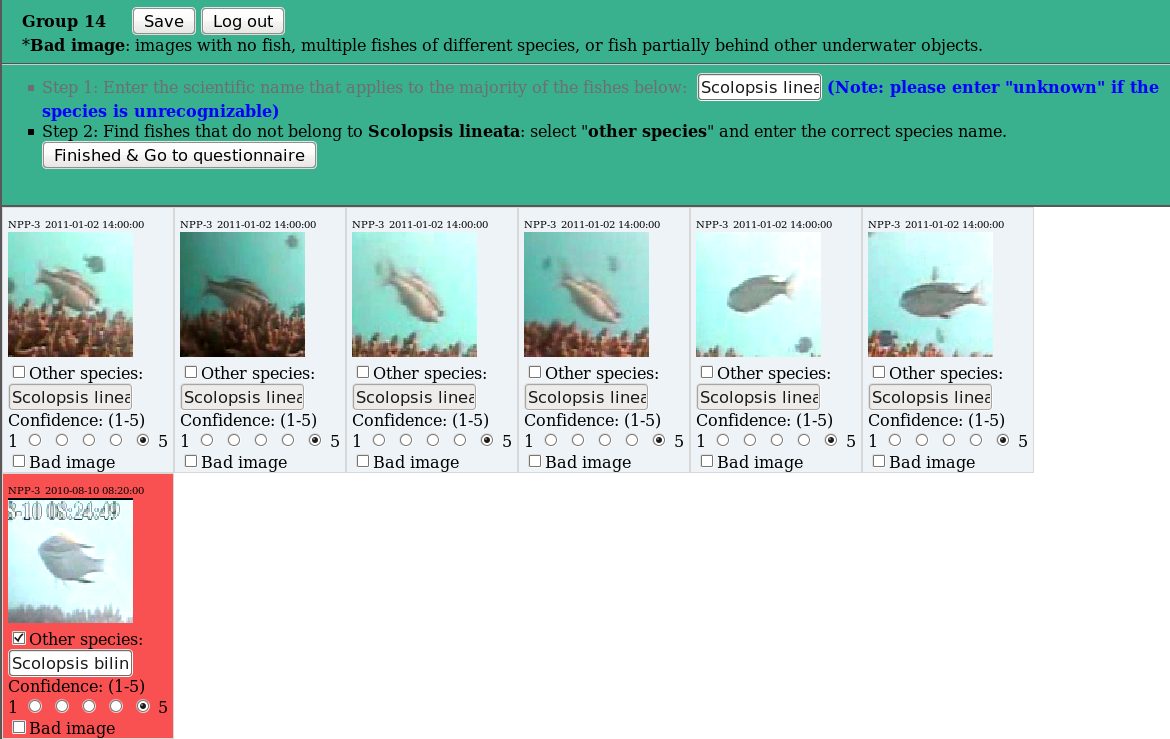
\includegraphics[width=0.48\textwidth, height=0.25\textwidth]{expertlabel.png}
\label{fig:expert_interface}
}
\subfigure[Game interface for non-experts]{
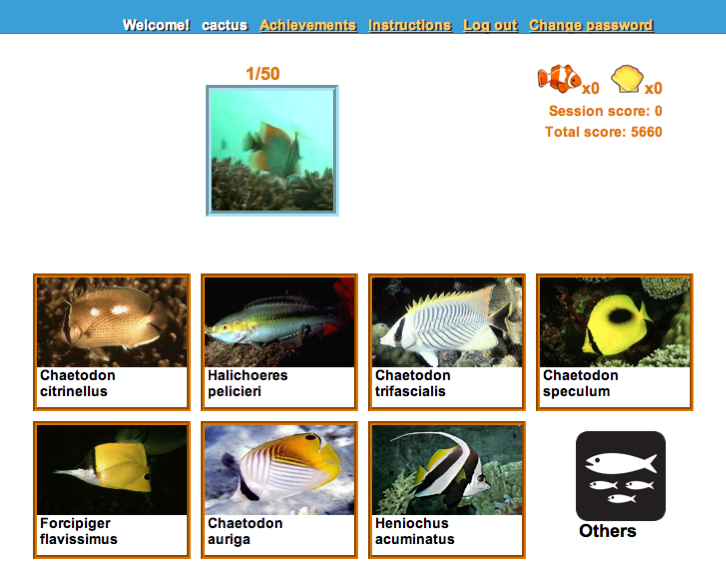
\includegraphics[width=0.45\textwidth, height=0.25\textwidth]{nonexpert_interface.png}
\label{fig:nonexpert_interface}
}
%\miniskip
\caption{Expert and game interfaces for labeling fish species.}
\end{figure*}

%==============OLD =======================================
\if 0
As already mentioned, experts are expensive and a scarce resource.
Therefore we ask our experts to label only a small subset of our data
and developed a cluster-based interface to facilitate their labeling
process. The images labeled by the experts are used as gold standard
for the evaluation of non-expert labels.

%\miniskip
\subsection{Experiment setup}
%
Two students manually clustered 3000 images randomly chosen from our
video data. The students were allowed to discuss and in total obtained
28 clusters. We present the images to the experts in a labeling
interface as shown in Figure~\ref{fig:expert_interface}. 
%
Using this interface, the expert first enters the species name that
applies to the majority of the images in a cluster. 
%in the top-right text box. 
Once the name is entered, all images within the cluster are
automatically assigned with the same species name. Then, the expert is
asked to select those images that should not belong to that cluster.
By selecting these images, he/she can also input the correct species
names for them. 
%for them in the text box under each image. 
In this manner, in the worst case, the expert will have to manually
assign a species name to each of the images, i.e., when the clustering
is so bad that each image within a cluster represents a different fish
species. In the best case, i.e., when the cluster is pure, the expert
only needs to enter the species name once.
%
After finishing annotation, we submit the expert to a questionnaire in
order to collect information such as whether the labeling task was
difficult for him/her, and why it was difficult. 
%
To limit the amount of effort experts need to examine the clusters, at
most 30 images are randomly selected from each cluster and shown to
the experts. As the size of the clusters is unevenly distributed,
e.g., only some of the clusters contain more than 30 images, we obtain
a total of 190 labeled images.

Since we collect experts' labels to create a gold standard, we need
experts to assign labels to the best of their ability. To this end we
put no constraints on the amount of time experts spent on the labeling
task or on the use of additional resources. In general experts were
able to recognize a fish based on their knowledge. For ``difficult"
species, they consulted textbooks to verify their judgement.  

\subsection{Data obtained}
%\label{subsec:exp_data}
We invited 3 marine biologists (referred to as E1, E2 and E3) to
participate in the expert labeling task. They have research experience
of 30, 10 and 25 years in Taiwanse coral reef fish, respectively. 
  
An analysis of the labels assigned by the experts to the 190 fish
images reveals that the biologists do not always agree on the species
names for an image.
%For 82.6\% of the images, at least two biologists agreed on a species
%name; for 56.3\% of the images, all biologists agreed on a name
%(including the cases where two biologists agreed on a species name
%while the third biologist indicated that he/she cannot identify the
%fish).
We use Cohen's kappa~\cite{Cohen60} to measure the agreement between
the expert labels, assuming the complete category set consists of all
unique species mentioned in the labels provided by the experts. 
%See Table~\ref{tab:expert_agree}.
\begin{table}[h!]
%\vspace*{-\baselineskip}
\centering
 \begin{tabular}{@{~}l@{~~~}l@{~~~}l@{~~~~~}l@{~~~}l@{~}}
 \hline
  & \multicolumn{2}{l}{Species level} & \multicolumn{2}{l}{Family level}\\
  Comparison & Avg.$\kappa$ & Sdv. & Avg.$\kappa$ & Stv.\\
  \hline
  E1 vs. E2  & 0.55 & 0.008 & 0.85 & 0.004\\
  E1 vs. E3  & 0.48 & 0.008 & 0.75 & 0.000\\
  E2 vs. E3  & 0.67 & 0.006 & 0.76 & 0.0001\\
  \hline
 \end{tabular}
  \caption{Cohen's kappa for measuring expert agreement.}
\label{tab:expert_agree}
%\vspace*{-\baselineskip}
\end{table}
%

In addition, we find that sometimes the biologists are not sure which
species a fish should belong to: 1) one of the experts assign labels
such as ``A or B'' to 3 images, and 2) in 45 cases (each case is a
pair of image and expert, in total we have 190 x 3 cases) a family or
higher level label is assigned. 
%39 genus
%For images with genus level labels there are no case where all 3 experts agree on a label.  
In the former case, we consider both labels mentioned, and in the
latter case, we consider all species under a higher level label as
possible target labels.  Thus it is possible that an image has
multiple labels assigned by a single expert.  In total, 288 species
and 20 families were mentioned as labels for the 190 images. 
%
Since Cohen's kappa does not handle multiple labels of a single rater,
we handle this situation as follows.\footnote{Notice that here we could
use other measures such as Fleiss' kappa to compute the agreement
between multiple raters. However we chose to use pairwise Cohen's
kappa for the following reason. In later experiment, we will compare
the agreement between aggregated non-expert labels and the expert
labels, to the agreement among the expert labels. In that case, we
will be comparing the agreement among 4 raters (3 experts and the
aggregated non-expert), to the agreement among 3 raters (3 experts).
The values of Fleiss' kappa calculated with different number of raters
are not comparable.} 
%First, we evaluate the agreement between labels at both species and family levels:
%it is expected that at family level, cases with such situation will be greatly reduced. 
%Second, 
When there exist multiple labels for an image assigned by one expert,
we randomly draw one of them as the target label being evaluated; we
repeat this process 100 times and report the averaged $\kappa$ and its
standard deviation over the 100 runs\footnote{Notice that the
agreement calculated in this way is rather conservative}. We evaluate
labels at both species and family level.

%
\begin{figure*}[t!]
\centering
\subfigure[Species recognition interface for experts]{
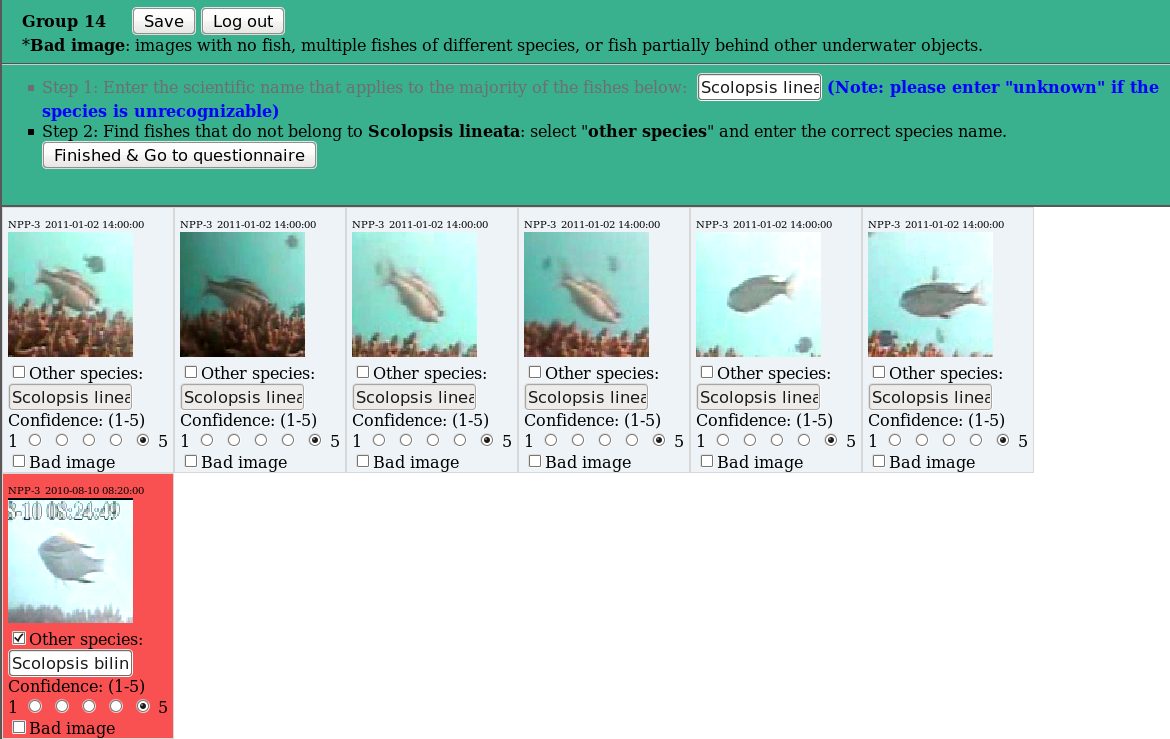
\includegraphics[width=0.48\textwidth, height=0.25\textwidth]{expertlabel.png}
\label{fig:expert_interface}
}
\subfigure[Game interface for non-experts]{
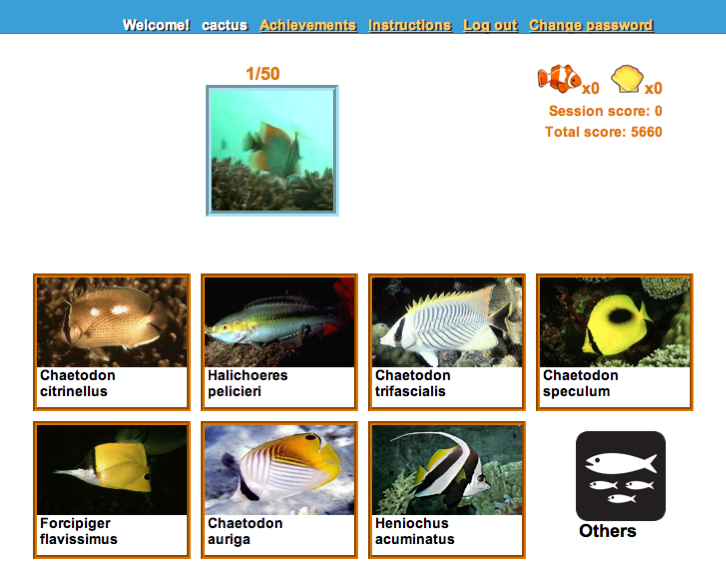
\includegraphics[width=0.45\textwidth, height=0.25\textwidth]{nonexpert_interface.png}
\label{fig:nonexpert_interface}
}
\caption{Expert and game interfaces for labeling fish species.}
\end{figure*}

Results in Table~\ref{tab:expert_agree} show that at the species
level, the agreement between experts is only moderate, while at family
level, a much stronger agreement can be found, but still not perfect.
This result suggests that our labeling task is not trivial even for
experts. 
%
Further, from the questionnaire we learn that according to the
experts, the top factors that make recognition difficult are: 1)~the
low quality of the images; and 2)~the fact that some species are
visually very similar and not distinguishable using the features that
can be observed from the images.  For example, the main feature
biologists use to distinguish Chromis Chrysura and Chromis
Margaritifer is their body size, while in video footage the size of a
fish depends on its distance to the camera, and therefore it does not
provide enough information. 
%

Note that we treat experts' labels as the ground truth. That is, if
two experts disagree, it does not mean that they make mistakes, but
that these species are not distinguishable given available
information.  The purpose of measuring the agreement between experts
is to provide a sanity check, or a (loose) upper bound for the
performance of the fish labeling task. 

\fi

 % a case study
\section{Labeling with non-experts}
\label{sec:nonexpt_label}


\subsection{Interface}
With the labeling interface presented in Fig.~\ref{fig:expert_interface},
%Section~\ref{sec:expt_label},  
it is very hard, if not impossible, for those who do not have knowledge with coral reef fish species to effectively provide labels. Therefore for non-experts a labeling interface as shown in Figure~\ref{fig:nonexpert_interface} is developed. 

The players are asked to compare a \textit{query image}, i.e., the image to be labeled, to  
a set of \textit{candidate labels}, i.e., textbook images of candidate species. 
They click a candidate label if they believe that the fish in that candidate label
and the query image belong to the same species, or ``others",  if none of the candidates is similar enough to be considered as the correct answer. 
%
A feedback score for the chosen label is provided. 
Ideally, players can learn from the feedback and improve their performance. 

%
The labeling process is divided into sessions of 50 query images. 
This gives a break as well as a goal for the players.  
It typically takes 5 to 10 minutes to complete a session. 
%, depending the player's familiarity with the system and the task.
%
To avoid overloading the players with too many candidates, we limit the number of candidates to 7. 
%
To increase user engagement with the labeling task, we show the top 10 scorers. 
%(those who have achieved 
%top scores in single sessions), and top contributors (those who have achieved accumulative top scores). 
This competition element is meant to encourage people to achieve higher scores and play more sessions. 

%\miniskip
\subsection{Experiment setup}
\label{subsec:nonexpt_exp}

%Recall that our first research question is: 
%\emph{with our proposed labeling strategy, can non-experts provide useful labels that are comparable to what experts can provide?} 
%\emph{
%Can non-experts achieve acceptable performance when compared 
%with the labels provided by the experts?
%}
%From the data obtained from the experts, 

%To answer our two research questions described in Section~\ref{sec:intro}, 
%we conduct two experiments that simulates two situations.

%\shrink
\subsubsection{Two simulated situations}
During the manual clustering stage, we find that 53 out of the 190 images 
were assigned to ``wrong" clusters. %during the manual clustering stage.  
That is, there exist many fish that look similar but belong to different species. 
Our first research question thus boils down to
 %
\emph{Can non-experts distinguish between similar species when examples of these species are displayed
next to each other?}
To find answers to this question, we conduct two experiments that simulate two situations. 
%

%\miniskip
\noindent
\textbf{Experiment 1.}
We first assume an ideal situation, where the \emph{target label(s)} (labels suggested by the biologists) 
of the query image is always among the candidates.
The primary goal of the experiment is to investigate whether the players can identify
the target label when there exist very similar species.

We select candidates that are similar to the target labels as follows.
%Recall that we have manually created clusters which are not always pure. 
Let $c=\{i_n\}_{n=1}^N$ be a cluster containing $N$ query images, and $f(i)$ maps an image
to one of the species $S=\{s_m\}_{m=1}^M$.
We compute a relevance score between an image $i \in c$ and a species as
%\begin{equation}
$\text{score}(i, s) = \text{count}(\{f(j) = s, j \in c\})/N$.
%\end{equation}
All species with a non-zero score are the ones that were clustered together, which means
that they are visually similar. We select top 7 species as candidates.
If less than 7 species were available, we fill the remaining slots with random images.
If more than 7 species have non-zero scores, 
%e.g., in case
%the biologists have assigned multiple labels to some of the images in the cluster, 
we make sure that the target labels are in the candidates.
%

%\miniskip
\noindent
\textbf{Experiment 2.}
We then consider a more realistic situation when some target labels are not in the candidates. 
%
%Notice the number of candidates is way smaller than the number of
%all possible fish species, e.g., 288 if we consider all the species mentioned by the biologists for the 190 images.
%
In practice, we do not have information about the target labels of the query images.
We need to select candidates based on certain similarity measures computed with automatic
methods, which are most likely imperfect. 
It is then important to know whether the non-expert players can still make right 
choice, that is, select ``others", when similar species are displayed as candidates. 
%
We use the same setting as in Expr.1 to select candidates and deliberately remove
the target labels from the candidates for a set of randomly selected query images. 
%On the one hand, we want sufficient cases where the target labels are removed, 
%on the other hand, 
Notice, if too many target labels are removed, users may
expect that ``others" is always the safe bet when they are not sure.   
With a few trial runs, we decide to remove the target labels for 25\% of the query images. 
%

%\shrink
\subsubsection{System feedback}
\noindent
%\textbf{Settings of feedback scores.}
%\label{subset:feedbacksetting}
%Apart from our main research question, we are also interested in 
Our second research question was: \emph{Can non-experts learn and improve their performance during the game?}

Players may be able to improve their performance for different reasons:
learning from the system feedback, getting used to the quality of the images, etc.
%They may for instance learn from the system feedback, get used to the quality of the images, etc.
In this study, we do not aim to identify \emph{why} and \emph{how} users improve, but focus on whether
they \emph{can} learn and improve. 
%
%We therefore only consider the simplest case for the system feedback,  i.e., feedback from the expert labels. 
%In this study, we only consider the simplest case for the system feedback, i.e., feedback from the expert labels.
Here we only consider the simplest and ideal system feedback, namely feedback from the expert labels.
%That is, under the ideal feedback setting, can users learn and improve over time?
Specifically, we assign scores to each click on an candidate label based on the biologists' voting, 
%Since experts do not always agree, 
i.e., a click on an option can receive 0, 1, 2, or 3 points.
%depending on the number of biologists agree that it is the target label. 
%
In practice when expert labels are not available, other types of feedback should be used, e.g., 
peer-agreement, automatic similarity measures. 
We leave questions such as how these feedbacks influence the user learning behavior to future investigation.
%are also very interesting research directions. We leave these for future investigation.


%\shrink
\noindent
\subsubsection{Aggregation of obtained labels}
%\label{subsec:data_nonexp}
We use convenience sampling to collect players. %non-expert annotators. 
We launched the game in our own social network and in public events, e.g., demo exhibitions. 
Our users have a diverse background and age groups, including school age children
as well as university students and researchers. 
%
We collect labels for the 190 images labeled by the experts.  %Avg.\#Label refers to the average number
22 players contributed 72 sessions in Expr. 1 and 32 players contributed 49 sessions in Expr. 2. 
On average each image received 19 and 13 labels, respectively.
%
%
Notice that in Expr. 2 we have more players but less sessions. This is because most
of the sessions of Expr. 2 were done in a public event, where people typically 
try out for just one session.  
%
Four players have participated both experiments and in total played 9 sessions in Expr. 2. 
In our evaluation of Expr. 2, we will treat their contributions separately, as they may have been 
trained in Expr. 1 and their performance is not comparable with those who were new to the game.

%\miniskip
%\noindent
%\textbf{Aggregating non-expert labels.}
%Since each query image is associated with multiple labels from multiple players, we 
%need to aggregate them into a single assignment for evaluation.
%
%While there exist many different approaches for aggregating labels, 
%here 
%We consider two simple strategies. 
%
%With the first strategy, we randomly select one of the players' labels as the chosen label for the query image. 
%If we run this random aggregation, say, 100 times, we obtain a sample of 100 label assignments given random labels from random %players.
%By evaluating the result of the randomly aggregated labels, we obtain an expected performance of a single player. 
%
%The second aggregation strategy is majority voting. 
%With majority voting, we can see if the crowd can help to cover individual' errors. 
To aggregate the labels from multiple players into a single label assignment for evaluation, we use
a simple majority voting strategy.
Since experts may give multiple labels to an image (as ground truth), 
we do not simply take the winner of the majority voting as the chosen label, but rank
the candidates in descending order of their votes.
%provide a rank of the candidates in descending order of their votes.
%
In Expr. 2 when target labels are not displayed and ``others" are \emph{correctly} chosen,
they do not provide information about which label should be assigned to the image.
We ignore these cases for aggregating as they neither hurt or help the performance. 


%=========OLD===========
\if 0
%\miniskip
\subsection{Interface}
For non-experts, a labeling game interface as shown in Figure~\ref{fig:nonexpert_interface} is used.
The players are asked to compare a \textit{query image} (i.e., the image to be labeled) to  
a set of \textit{candidate labels}, i.e., labeled images of candidate species.
%
%where the category images are the textbook examples of fish species 
%\footnote{We call a fish species or family a ``category". When evaluating the user
%performance, we consider categories in both species and family levels; when showing candidate
%categories, we only consider species level, as it is the lowest level in taxonomy of the biological classification.}. 
%
To avoid overloading the players with too many candidates, we limit
the number of candidates to 7. 
They choose from one of the candidates if they believe that the fish in that candidate label
and the query image belong to the same species, or ``others",  if none of the candidates is similar enough to 
be considered as the correct answer. The labeling task is then a multiple choice based on 
the perceived visual similarity between the query image and the candidate label images. 
%
The player receives a feedback score for each choice he/she makes. 
Ideally, he/she can learn from the feedback and tries to improve his/her performance. 

We divide the labeling process into sessions of 50 query images. 
This gives a break as well as a goal for the players.  
It typically takes 5 to 10 minutes to complete a session, depending on whether the player is familiar with the 
system and the task.

In order to increase user engagement with the labeling task, we included competition
elements. We show the top 10 scorers (those who have achieved top scores in single sessions),
and top contributors (those who have achieved accumulative top scores), which is meant to encourage
people to achieve higher scores and play more sessions.


%\miniskip
\subsection{Experiment setup}
\label{subsec:nonexpt_exp}
Recall that our first research question is: 
%\emph{with our proposed labeling strategy, can non-experts provide useful labels that are comparable to what experts can provide?} 
%\emph{
Can non-experts achieve acceptable performance when compared 
with the labels provided by the experts?
%}

%From the data obtained from the experts, 
We find that 53 out of the 190 were assigned to ``wrong" clusters during
the manual clustering stage.  That is, there exist many fish that look similar but do not belong to the same species. 
The question thus boils down to
 %
\emph{Can non-experts distinguish between similar species when examples of these species are displayed
next to each other?}
%
To find answers to this question, we conduct two experiments that simulates two situations. 
%

%\miniskip
\subsubsection{Experiment 1}
We assume an ideal situation, where the \emph{target label(s)}, i.e., labels suggested by the biologists,  
of the query image is always among the candidates.
The primary goal of the experiment is to investigate whether the players can identify
the target label when there exist very similar species.

We select candidates that are similar to the target labels as follows.
Recall that we have manually created clusters which are not always pure. 
Let $c=\{i_n\}_{n=1}^N$ be a cluster containing $N$ query images, and $f(i)$ maps an image
to one of the species $S=\{s_m\}_{m=1}^M$.
We compute a relevance score between an image $i \in c$ and a species as
%\begin{equation}
$\text{score}(i, s) = \text{count}(f(c) = s)/N$.
%\end{equation}
All species with a non-zero score are the ones that were clustered together, which means
that they are visually similar. We select top 7 species as candidates.
If less than 7 species were available, we fill the remaining slots with random images.
If more than 7 species have non-zero scores, e.g., in case
the biologists have assigned multiple labels to some of the images in the cluster, we make sure that
the target labels are in the candidates.
%
%
%\miniskip
\subsubsection{Experiment 2}
%In this experiment, we investigate whether the non-experts can make correct decision
%when the target labels are not in the candidates.
We now consider a more realistic situation when some target labels are not in the candidates. 
%
Notice the number of candidates is way smaller than the number of
all possible fish species, e.g., 288 if we consider all the species mentioned by the biologists for the 190 images.
%
In practice, we do not have information about the target labels of the query images.
We need to select candidates based on certain similarity measures computed with automatic
methods, which are most likely not perfect. 
It is then important to know whether the non-expert players can still make right 
choice, i.e., select ``others" when similar species are displayed as candidates. 

We use the same setting as in Expr.1 to select candidates and deliberately remove
the target labels from the candidates for a set of randomly selected query images. 
On the one hand, we want sufficient cases where the target labels are removed, 
on the other hand, if too many target labels are removed, the users may
expect that ``others" is always the safe bet when they are not sure.   
With a few trials, we decide to remove the target labels for 25\% of the query images. 
%

%\miniskip
\subsubsection{Settings of feedback scores}
%\label{subset:feedbacksetting}
%Apart from our main research question, we are also interested in 
Our second research question was: To which extent can the non-expert players learn their performance during the game?
%\emph{Can non-expert improve their performance over time?}

%Intuitively, we expect that users learn from the system feedback scores given that they would aim to achieve higher scores.
%There are however more than one reason why the annotators may be able to improve their performance. 
The players may be able to improve their performance for a number of reasons.
%E.g., they may learn from the system feedback,  may get used to the quality of the images over time and are able to observe more details. 
They may for instance learn from the system feedback, get used to the quality of the images, etc.
In this study, we do not aim to identify \emph{why} and \emph{how} users improve, but focus on whether
they \emph{can} or \emph{cannot} learn and improve. 

%We therefore only consider the simplest case for the system feedback,  i.e., feedback from the expert labels. 
In this study, we only consider the simplest case for the system feedback, i.e., feedback from the expert labels.
That is, under the ideal feedback setting, can users learn and improve over time?
Specifically, we assign scores to each option of the candidates based on the biologists' voting. 
Since experts do not always agree, a click on an option can receive 0, 1, 2, or 3 points, 
depending on the number of biologists agree that it is the target label. 

In practice when expert labels are not available, of course, other types of feedback should be used, e.g., 
peer-agreement, automatic similarity measures. 
We leave questions such as how these feedbacks influence the user learning behavior to future investigation.
%are also very interesting research directions. We leave these for future investigation.

%\miniskip
\subsection{Data obtained}
%\label{subsec:data_nonexp}
We use convenience sampling to collect our players. %non-expert annotators. 
We launched our game in our own social network as well as in public events, e.g., demo exhibitions. 
Our users have a diverse background and age groups, including school age children
as well as university students, researchers, etc. 
%
We collect labels for the 190 images that are labeled by the experts.  %Avg.\#Label refers to the average number
22 players contributed 72 sessions in Expr. 1 and 32 players contributed 49 sessions in Expr. 2. 
On average each image received 19 and 13 labels, respectively.
%
%\begin{table}[h!]
%\vspace*{-\baselineskip}
%\caption{Statistics of the collected labels. }
%\centering
%\begin{tabular}{lccc}
%\hline
%Experiment & \#Users & \#Sessions & Avg.\#Labels per image\\
%\hline
%1 & 22 & 72 &  19\\
%2 & 32 & 49 &  13\\
%\hline
%\end{tabular}
%\label{tab:stats_label}
%\vspace*{-\baselineskip}
%\end{table}
%
Notice that in Expr. 2 we have more players but less sessions. This is because most
of the sessions of Expr. 2 were done in a public event, where people typically 
try out for just one session.  
%
%Therefore when studying the learning effect of users, we only consider the labels collected in the first experiment. 
%In Experiment 2, among the 32 annotators, 
%
Four players have participated both experiments and in total played 9 sessions in Expr. 2. 
In our evaluation of Expr. 2, we will treat their contributions separately, as they may have been 
trained in Expr. 1 and their performance is not comparable with those who were new to the game.

%\miniskip
\subsection{Aggregating non-expert labels}
Since each query image is associated with multiple labels from multiple players, we 
need to aggregate them into a single assignment for evaluation.
%
%While there exist many different approaches for aggregating labels, 
%here 
We consider two simple strategies. 

With the first strategy, we randomly select one of the players' labels as the chosen label for the query image. 
If we run this random aggregation, say, 100 times, we obtain a sample of 100 label assignments given random labels from random players.
By evaluating the result of the randomly aggregated labels, we obtain an expected performance of a single player. 
%
The second aggregation strategy is majority voting. 
%With majority voting, we can see if the crowd can help to cover individual' errors. 
Since experts may give multiple labels to an image, 
we do not simply take the winner of the majority voting as the chosen label, but rank
the candidates in descending order of their votes.
%provide a rank of the candidates in descending order of their votes.

In Expr. 2 when target labels are not displayed, the labels ``others" can be correct
but not providing information about which label should be assigned to the image.
% label ``others'' can be correct but does not provide
%actual information about which label should be assigned to the image, i.e., in case
%that the target labels are not displayed. 
We ignore these labels when aggregating as they neither hurt or help the performance. 

\fi
%\subsection{Aggregating non-expert labels}
%\label{subsec:agg_nonexp}
%After rounds of annotation, each image is attached with a set of labels by a number of annotators.
%We then need to aggregate these annotations into a coherent assignment of labels. 
%Preferably the aggregated labels is consistent with the labels provided by the marine biologists.
%As we have already seen, an image can have multiple possible labels according to the expert judgements, 
%some are more preferable than others.
%When aggregating the non-expert annotations, similarly, we allow an image to be assigned to multiple categories
%and meanwhile aim to obtain an estimation of how likely a category is relevant to the image (or in other word, is
%the correct target label for that image).
%%
%Ideally, the aggregated non-expert labels matches expert labels. For example, the category that is most likely to be 
%the target label according to the non-experts is also the most preferred label according to the experts.
%
%
%Let us start with a more formal statement of the problem. 
%For an images $i$ and a set of categories (i.e., fish species or family names) $C_i=\{c_j\}_{j=1}^N$, the goal
%is to assign ``relevance'' scores to each $(i, c)$ pairs, where $c \in C$ and $i \in I$ that indicates how likely a category $c$
%is the correct answer for image $i$.  For simplicity, we only consider candidate categories that has been judged at least once. 
%
%When annotating an image,  each annotator sees a set of candidate categories $C_i=\{c_k\}_{k=1}^K$, 
%where $k<<N$. The annotator is asked to pick the one that they think is most likely to be the correct answer.
%We consider two ways to aggregate the labels from multiple annotators (as well as the labels provided by the same annotator
%but at different time points). 
%
%\subsubsection{Voting}
%The first method we consider is a simple voting approach.
%Specifically, we define the relevance score of a category $c$ with respect to image $i$ as the number of times
%$c$ is selected as the target label for $i$ out of the number of time $c$ and $i$ are shown together to be judged, 
%\begin{equation}
% s(c, i) = \frac{count(c^*= c, i)}{count(c, i)},
%\end{equation}
%where $c^*$ is the category selected by the annotator as the target label.   
%That is, when $c$ and $i$ are shown together to the annotators, 
%the more often category $c$ is chosen to be the target label for image $i$, the more likely that $c$ is relevant to $i$.
%
%
%\subsubsection{Maximum a posteriori (MAP) estimation}
%\todo{Why is it better than voting? because voting is not robust against random noise}
%
%Notice that in our set-up, the annotators do not see the whole set of candidates and therefore the labels they give only provide
%their preference among the $k$ candidates. Hence, instead of treating each label as an independent assignment
%of a category to an image, it is probably more appropriate to treat it as a comparison between the $k$ candidate categories.
%That is, the selected category $c^*$ is the most likely correct answer \textit{relative} to the other $k-1$ candidates.
%
%To convert the (incomplete) preference judgements from multiple annotators to a single scale rating of the relevance scores
%between the candidate categories and the image, we follow Thurstone's Case V Model~\cite{thurstone27:alaw}.
%
%Let $r_{k, i} \sim \mathcal{N}(\mu_{k, i}, \sigma_{k, i}^2)$ and $r_{l, i} \sim \mathcal{N}(\mu_{l, i}, \sigma_{l, i}^2)$
%be the distribution of the true relevance of two categories $c_k$ and $c_l$ with respect to image $i$.  
%For simplicity, in the rest of the section,
%we will drop all the $i$'s and keep in mind that all the discussion is with respect to a specific image $i$.
%
%For a category $c$, the mean of its corresponding Gaussian $\mu_c$ is taken to be its \textit{relevance score}.
%%
%The \textit{relevance} of a category, on the other hand, is assumed to be a Gaussian random variable, since the annotators' judgements
%are subjective: different people, or perhaps a same person at different times,  may have different opinions about the relevance
%of the same pair of $(c, i)$. 
%%
%According to Thurstone's model, when the annotators judge whether category $k$ is better than $l$, 
%%a realization of the relevance of $c_k$ and $c_l$ is drawn from each of the relevance distributions and the option with the higher relevance is chosen. 
%they sample a realization of the relevance difference from the distribution 
%\begin{equation}
%r_{k}-r_{l} \sim \mathcal{N}(\mu_{kl}, \sigma_{kl}^2), 
%\end{equation}
%where $\mu_{kl} = \mu_k - \mu_l$, and $\sigma_{kl}^2$ is the variance of the difference of random variables $k$ and $l$. 
%% 
%They choose $k$ over $l$ if $p(r_k - r_l > 0)$,  and we have
%%
%\begin{equation}
%%\mu_{kl} = \sigma^2_{kl}\mathrm{\Phi}^{-1}(p(r_k - r_l)), 
%p(r_k-r_l > 0) = \mathrm{\Phi} (\frac{\mu_k - \mu_l}{\sigma_{kl}}) 
%\end{equation}
%where $\mathrm{\Phi}$ is the inverse cumulative density function (CDF) of the standard normal distribution.
%%
%Further, with the Case V assumptions, i.e., equal variance and zero correlation of $k$ and $l$, $\sigma^2_{kl}$ can be 
%set to 1~\cite{thurstone27:alaw, tsukida11:how}.
%For more details of the derivation of the equations we refer to~\cite{tsukida11:how}.
%
%Now back to our original problem, where we have $N$ candidate categories with unknown relevance scores $\mu=[\mu_1, ..., \mu_n]$. 
%Our goal is to find an assignment of $\mu$ that fits best with our annotated data. 
%%
%We employ a maximum a posteriori estimation, which has shown reliable performance compared to many other approaches~\cite{tsukida11:how}.
%
%We first convert the result of the annotation to preferences of one category over another.
%For example, if $c_1$ is selected among candidates $c_1$, $c_2$ and $c_3$, we have preferences $c_1>c_2$ and $c_1>c_3$.  
%We store the counts of such preference aggregated from multiple judgements in a matrix $M$. 
%% 
%\begin{equation}
%   m_{ij} =
%   \begin{cases} 
%   \textit{count}(c_i > c_j),  & i \ne j, \\
%   0,  & i=j.
%    \end{cases}	
%\end{equation}
%%
%Then, following~\cite{tsukida11:how}, to find the maximum a posteriori assignment, we solve the following optimization problem: 
%\begin{equation}
% \begin{split}
%\arg\max_{\mu}  & \sum_{k, l} M_{k,l}  \log(\mathrm{\Phi} (\mu_k - \mu_l) ) - \sum_k \frac{\mu_k^2}{2},\\
%\text{subject to}   & \sum_k \mu_k = 0,
%\end{split}
%\end{equation}
%where the first term of the objective function is the log-likelihood of $\mu$ given our annotated data, and
%the second term is a Gaussian prior. The constraint makes sure that the assignment is unique. 












 % a case study
\subsection{Evaluation}
%To measure the performance of non-expert, 
\noindent
\textbf{Quality of non-expert labels.}
We use Cohen's $\kappa$ to measure the agreement between the 
aggregated non-expert labels and each of the three experts. 
We compare these to the pairwise agreement among the experts. 
When using majority voting, we take the top 1 candidate as the chosen label. 
In the case of ties, we use the same approach as described in Section~\ref{sec:expt_label} to 
calculate the agreement. 

Further, NDCG~\cite{Jarvelin02:ndcg} is used %as an alternative measure, 
as it provides an intuitive interpretation of the correctness of the labels.
For a query image, given the biologists' voting, each candidate can be rated as 0, 1, 2, or 3. 
The ranked list of candidates as a result of majority voting
%generated by the (majority) voting aggregation 
is then evaluated using these graded expert judgements.

\noindent
\textbf{Learning behavior of non-expert users.}
%We study two types of learning behaviors: 
%whether the players' performance improves over time
We study users' performance over time in terms of  
1)~memorization: when an image is shown again;
and 2)~generalization: when an unseen image that belongs to a seen species is shown.

%1)~memorizing: whether the players' performance improves
%over time when an image is shown again;
%and 2)~generalization: whether the players' performance
%improves regarding different images that belong to the same species.  

We measure the performance of a single label as follows. 
Let $L=\{l_k\}_{k=1}^K$ be the candidate labels for an image, 
$J(l)=\{0, 1\}$ be a player's judgement, 
and $E(l)=\{0, 1, 2, 3\}$ be the expert votes of label $l$ for the image. 
The performance of a judgement is defined as
experts' votes for the chosen candidate normalized by the
maximum votes one can achieve for the set of candidates:
%
%\begin{equation}
 $s =  \frac{\sum_{l \in L} J(l) \cdot E(l)}{\max_{l \in L} E(l)}$. 
 %\label{eq:score}
%\end{equation}
%
%That is, 
%
Since scores achieved at a certain time point can be sensitive to players' random errors, 
we smooth the score at each time point with the scores achieved so far:
$s_t = \sum_{i=1}^t s_i / t$.
%
%In practice, 
$t$ refers to the $t$th time a player labels the same image (memorization), or a different image in the same species (generalization). 
%
%If a player has labeled an image $i$ (or images from species $i$) for $t$ times, we call it a repetition 
%(or generalized repetition) with $t$ labels. 
%By comparing the scores defined above at different $t$, 
%we can observe whether the non-expert performance improves over time.

%In order to have images shown multiple times to a player,  
In a session, the first 12 images are randomly selected without repetition. 
After that, with a probability of 0.5 
an image is selected
from those that were already labeled in the current session. 
%
As images are selected randomly, the repetition of images (memorization) or 
species (generalization) do not happen the same number of times. 
In order to conduct reliable statistical testing for comparison %(Wilcoxon rank-sum test %~\cite{Wilcoxon45} 
(see Section~\ref{sec:res}), we consider repetitions of images/species 
that have more than 30 cases\footnote{A case is a $\{\textit{image(species), user}\}$ pair.}. 
Specifically, we consider $\le 4$ repetitions of images for both experiments; 
$\le 25$ repetitions of species for  Expr. 1, and $\le 10$ for Expr. 2.
As fewer sessions were played in Expr. 2, less repetitions are available. 

%If a player has labeled an image $i$ (or images from species $i$) for $t$ times, we call it a repetition 
%(or generalized repetition) with $t$ labels. 
%Since images are selected randomly, 
%the repetitions or generalized repetitions do not happen the same number of times. 
%%E.g., in Expr. 1, we have 325 cases of repetition with 2 labels, but only 14 cases of repetition with 5 labels. 
%In order to be able to conduct reliable statistical testing for comparison %(Wilcoxon rank-sum test %~\cite{Wilcoxon45} 
%%in this case), 
%we only consider repetitions that have more than 30 cases.  
%We set $t \le 4$ for memorization for both experiments; 
%$t \le 25$ for generalization in Expr. 1 and $\le 10$ in Expr. 2, 
%as fewer sessions were played in Expr. 2 and therefore less repetitions are available.


%=========OLD==========
\if 0
\section{Evaluation}
\label{sec:eval}
%
%As discussed in Section~\ref{sec:intro}, the main questions with respect to our approach
%are i)~whether the non-experts can achieve a reasonable performance under such a setup; and ii)~whether non-experts
%users can learn from the system feedback on their annotation and improve their performance during this process.
%In order to answer these questions, we conduct a set of experiments to analyse the effectiveness of the proposed
%labeling strategy as well as the non-expert user behaviour under it.

%We evaluate the results from the game by measuring expert and non-expert agreement, 
%game-based ranking in terms of NDCG and learning effects.
%\miniskip
\subsection{Non-expert agreement with experts}
One natural way to evaluate the non-expert performance is to measure
the agreement between the non-expert labels and the expert labels.
%
%annotation is to measure the agreement between
%the labels given by the experts and those given by the non-experts. 
Again, we use Cohen's kappa~\cite{Cohen60}.  %as an agreement measure. 
%
%While there exist certain commonly used interpretation of the $\kappa$ values, e.g., a $\kappa$ value above
%0.6 is considered as a strong agreement, within our specific context, it is not obvious whether
%the non-expert performance is ``reasonable'' or not given a single $\kappa$ value.
%
Recall that in Section~\ref{sec:expt_label} we have already seen that the marine biologists often disagree on 
the species names % for a given image 
among themselves. 
% If the experts cannot agree on their labels, it is probably unreasonable to require the non-experts achieve an extremely high agreement with the experts. 
%
%In order to obtain a more tangible result of the non-expert performance, we ask the following question:
% We therefore ask the question: How does the agreement between non-experts and experts compare to the agreement between experts?

%Specifically, 
We measure the agreement between the aggregated non-expert labels and each of the 
three experts. We compare these to the pairwise agreement among the experts. 
When using majority voting, we take the top 1 candidate as the chosen label. 
In the case of ties, we use the same approach as described in~\ref{sec:expt_label} to 
calculate the agreement. 

%In addition, we create a set of aggregated expert labels and compare it to both experts' and non-experts' labels.
%
%To aggregate the experts' labels, we use majority voting and take the categories 
%\footnote{It is possible that multiple categories get same number of votes due to the fact that experts sometimes assign multiple
%categories to the same image.} 
%with the highest votes as the aggregated labels.
%
%On the other hand, for the aggregated non-expert labels, we also take the categories with highest scores
%as target labels.



%As we have discussed already, it is possible that an image has multiple labels assigned by a single expert or 
%the aggregated non-expert, while Cohen's kappa does not handle multiple labels.
%We handle this situation as follows. First, we evaluate the agreement between labels at both species and family levels:
%it is expected that at family level, cases with such situation will be greatly reduced.
%Second, when there exist multiple labels for an image assigned by one expert, we randomly draw one of the them as the 
%target label being evaluated; this process is repeated 100 times and we report the averaged $\kappa$ and its standard deviation
%over the 100 runs. Note that the agreement calculated in this way is rather conservative. 

%\miniskip
\subsection{Non-expert performance in terms of NDCG}
\label{subsec:eval_ndcg}
While the agreement analysis provides us with insights of the alignment between non-experts and experts,
% in comparison with
%the expert-expert agreement as a baseline, 
it does not provide an intuitive indication of how correct the obtained labels are. 
Further, we do not have a  principled way to handle the multi-label situation with $\kappa$.

We therefore also evaluate using of NDCG~\cite{Jarvelin02:ndcg}, which handles multi-labels
and provides a more intuitive interpretation of the correctness of the labels. 
For a query image, given the biologists' judgment, each candidate can be rated as 0, 1, 2, or 3. 
%These are used as the ground truth with graded judgements. 
The ranked list of candidates generated by the (majority) voting aggregation is then evaluated using
this grated expert judgements.

%We therefore provide an evaluation of the non-expert labels in terms of their correctness.
%We use the expert labels as ground truth. For an image, we consider the number of votes of a candidate
%category given by the experts an indication of the relevance of the candidate category to the image. 
%
%Specifically, we have three marine biologists and therefore each image-category pair can be rated $\{0, 1, 2, 3\}$.
%On the other hand, we aggregate the non-expert labels using the two methods as described in~\ref{subsec:agg_nonexp}, 
%which result in ranked lists of categories in descending order of their scores. 
%
%Given the graded relevance judgement and the ranked list of non-expert labels, we use NDCG~\todo{REF} as the 
%evaluation metric. 

%\todo{
%In addition, we are interested in when we can expect the non-expert labels to be reliable. 
%Some images are easier than others for annotators to provide accurate labels, e.g., some species may have unique features, 
%some images are of better qualities, etc. 
%We hypothesize that for easy images, it is more likely to have high agreement among annotators, as it is easier
%to find the correct labels, while for ``difficult'' images the annotators may provide diverse labels as it is hard to determine
%the correct answer. 
%We validate the hypothesis by measuring the Pearson correlation~\todo{REF} between two quantities, namely, 
%the NDCG scores, and the entropy of the non-expert labels of the images.
%Let $C_i$ be all the categories assigned to image $i$, the entropy of the labels is calculated as
%\begin{equation}
% H_i = -\sum_{c_i \in C_i} p(c_i) \log p(c_i),
%\end{equation}
%where $p(c_i)$ is defined as $\textit{count}(c_i)/\textit{count}(C_i)$.
%}

%\miniskip
\subsection{Learning behaviour}
%\label{subsec:eval_learn}
%As described in Section~\ref{sec:nonexpt_label}, we provide feedback to the non-expert annotators. 
%Intuitively, if the annotators can learn from the feedbacks they received, their performance
%would improve over time. For example, when seeing an image that has appeared before, one may be able to 
%remember the choice he/she made before and try to make an correction if it was wrong or stick to it when it was correct,
%given that his/her goal is to maximize his achievement score in our game setup. 

We investigate two types of learning behaviors: 
1)~memorizing: whether the players' performance improves
over time when an image is shown repeatedly (but not continuously);
and 2)~generalization: whether the players' performance
improves regarding different images that belong to the same species.  

We measure the performance of a single label as follows. 
Let $L=\{l_k\}_{k=1}^K$ be the candidate labels for an image, 
$J(l)=\{0, 1\}$ be the judgement given by a player, 
and $E(l)=\{0, 1, 2, 3\}$ be the expert votes of label $l$ for the image. 
The performance of a single judgement is computed as
%
\begin{equation}
 s =  \frac{\sum_{l \in L} J(l) \cdot E(l)}{\max_{l \in L} E(l)}. 
 \label{eq:score}
\end{equation}
%
That is, the expert votes for the selected candidate,  normalized by the
maximum votes one can achieve for the set of candidates $L$.
%
%Players may make random mistakes and %at some point and %therefore 
%scores achieved at certain time point can be sensitive to such mistakes. 
Since scores achieved at a certain time point can be sensitive to the players' random errors. 
we smooth the score at each time point with the scores achieved so far, i.e., 
$s_t = \sum_{i=1}^t s_i / t$.
%Specifically, at time $t$, we average over the scores achieved up till $t$ as the score at point $t$:
%\begin{equation}
 % s_t = \frac{1}{t}\sum_{i=1}^{t}s_i.
 % \label{eq:score_t}
%\end{equation}

In practice, $t$ refers to the $t$th time a player labels the same image, (or a different image in the same species). 
If a player has labeled an image $i$ (or images from species $i$) for $t$ times, we call it a repetition 
(or generalized repetition) with $t$ labels. 
By comparing the scores defined above at different $t$, 
%computed using Eq.~\ref{eq:score} and~\ref{eq:score_t} at different $t$, 
we can observe whether the non-expert performance improves over time.

In order to have images shown multiple times to a player,  in each session, 
we randomly select first 12 images without repetition. After that, with a probability of 0.5
we select an image from the ones that were already labeled in the current session. 
%
Since images are selected randomly, 
%If a user has labeled an image $i$ (or images from species $i$) for $x$ times, we call it 
%a case of repetition (or generalized repetition in the case of  generalization) of $x$ labels.
%Since images are selected randomly during the labeling process as described in Section~\ref{subsec:eval_learn},
the repetitions or generalized repetitions do not happen for the same number of times. 
E.g., in Expr. 1, we have 325 cases of repetition with 2 labels, but only 14 cases of repetition with 5 labels. 
In order to be able to conduct reliable statistical testing for comparison (Wilcoxon rank-sum test~\cite{Wilcoxon45} in this case), 
we only consider repetitions that have more than 30 cases.  
We set $t=1, ..., 4$ for memorization for both experiments; 
$t=1, ..., 25$ for generalization in Expr. 1 and $1, ..., 10$ in Expr. 2, 
as fewer sessions were played in Expr. 2 and therefore less repetitions are available.
%For memorization, with both experiments, we consider $t = 1, ..., 4$.
%For generalization, with Expr. 1, we consider $t = 1, ..., 25$, and with Expr. 2, we consider $t  = 1, ..., 10$, 
%as fewer sessions were played in Expr. 2 and therefore less repetitions are available. 
%See Section~\ref{subsec:res_learn} for detailed results. 

%For memorization, with both experiments, we consider repetition of 1, 2, 3, and 4 labels. 
%For generalization, with Experiment 1, we consider generalized repetitions of 1 to 25 labels, and with experiment 2, 
%we consider generalized repetitions of 1 to 10 labels, as fewer sessions were played in Experiment 2 and therefore
%less repetitions are available. 

\fi









 % evaluation 
\section{Results and discussion}
\label{sec:res}
%\miniskip
\noindent
\textbf{Performance of non-experts.}
\begin{table}[t!]
\centering
%\resizebox{\textwidth}{!}{
%\begin{tabular}{@{}l@{~~}l@{~~}l@{~~~}l@{~~}l@{~~~}l@{~~}l@{~~~}l@{~~}l@{~~~}l@{~~}l@{~~~}l@{~}l@{}}
\caption{Agreement between experts and non-experts. } 
\begin{tabular}{@{}l@{~~}l@{~~}l@{~~~}l@{~~}l@{~~~}l@{~~}l@{~~~}l@{~~}l@{~~~}l@{~~}l@{~~~}l@{~}l@{}}
\toprule
%& \multicolumn{6}{c}{Species} & \multicolumn{6}{c}{Family} \\
& & \multicolumn{2}{c}{E1} & \multicolumn{2}{c}{E2} & \multicolumn{2}{c}{E3}\\ 
%& \multicolumn{2}{c}{E1} & \multicolumn{2}{c}{E2} & \multicolumn{2}{c}{E3} \\
& & Avg. $\kappa$ & Sdv. & Avg. $\kappa$ & Sdv. & Avg. $\kappa$ & Sdv. \\
%& Avg. $\kappa$ & Sdv. & Avg. $\kappa$ & Sdv. & Avg. $\kappa$ & Sdv.\\
\hline
%U.random & 0.51 & 0.03 & 0.53 & 0.03 & 0.45 & 0.03     & 0.73 & 0.03 & 0.71 & 0.03 & 0.62 & 0.03\\ 
Expr.1 & Species & 0.62 & 0.01 & 0.65 & 0.006 & 0.55 & 0.009 \\  
& Family & 0.83 & 0.008 & 0.81 & 0.01 & 0.72 & 0.009\\
\hline
Expr.2 & Species & 0.65 & 0.009 & 0.50 & 0.008 & 0.45 & 0.009\\
(New)& Family & 0.73 & 0.01 & 0.73 & 0.01 & 0.68 & 0.01\\
\hline
Expr.2 & Species &0.53 & 0.01& 0.68 & 0.01 & 0.64 & 0.02 \\
(Old)& Family & 0.80 & 0.02 & 0.78 & 0.02 & 0.74 & 0.01\\
\bottomrule
\end{tabular}
%}
%(correct labels present).}
\label{tab:agree1}
%\vspace*{-\baselineskip}
\end{table}
%
Table~\ref{tab:agree1} shows the result of label agreement
at both species and family level. 
In terms of Expr.1, 
%
if we compare Table~\ref{tab:agree1} to Table~\ref{tab:expert_agree}, 
%we see that even with a random aggregation, 
we see that the agreement between expert and non-expert labels are rather similar to that among the experts themselves.
%
In terms of Expr.2, we see that the ``new" players (those who only participated in Expr.2)
achieve lower agreements with experts compared to players in Expr.1. 
%
%On the other hand, 
while the performance of ``old'' players is comparable to that of Expr.1.
This to some extent suggests that although the experimental condition has changed, 
the ``training" the players received during Expr.1 has an influence on their performance in Expr.2. 

\begin{table}[t!]
%\vspace*{-\baselineskip}
\centering
\caption{Non-experts' performance evaluated by NDCG.
\dubbelop(\dubbelneer) indicates a significant difference (p-value$<0.01$) tested using Wilcoxon signed-rank test.}
\begin{tabular}{@{}l@{~~}l@{~~}l@{~~}l@{~~}l@{}}
\toprule
 Method & \multicolumn{2}{c}{Species} & \multicolumn{2}{c}{Family}\\
 & NDCG@1 & NDCG@5  & NDCG@1 & NDCG@5\\ 
 \hline
 Expr.1 & 0.84 & 0.88 & 0.93 & 0.94\\
\hline
Expr.2.new & 0.72\dubbelneer  & 0.77\dubbelneer  & 0.86\dubbelneer & 0.94\\
Expr.2.old & 0.88 & 0.86 & 0.91& 0.94\\
\bottomrule
\end{tabular} 
\label{tab:ndcg}
%\vspace*{-\baselineskip}
\end{table}


Further, Table~\ref{tab:ndcg} shows the performance of non-expert labels in terms of NDCG. 
%
In practice, when using the collected labels as training data, often only the label(s) with 
the highest scores are considered as target labels. 
%
Thus it is important that the top ranked labels are correct according
to experts' labels. We list the results of NDCG@1 and 5.  
Unlike the agreement comparison, here we do not 
% directly interpret the results as ``reasonable" or not, 
% as we do not 
have a baseline to compare to.  However, we do see that the scores at least
indicate that for a majority of the images, the non-experts have made correct choices. 
%Since random aggregation only has one chosen label, below NDCG@1, 
%no further gain can be achieved. For majority voting, we see that some other
%relevant candidates are within the top 5 of the ranked list, as the
%scores at NDCG@5 are higher than that at NDCG@1. 
%
%Intuitively, this is a more difficult task for the players, as we deliberately removed
%the target labels of some of the query images, and left in candidates that are similar but not actually relevant. 
%Table~\ref{tab:ndcg2} lists the results in terms of NDCG. 
The new players in Expr.2 have a significant lower performance compared to
Expr.1, while the performance of ``old" users do not show significant difference compared to 
that achieved in Expr.1. 
%both with random aggregation and majority voting. 
%The differences are statistically significant. 
%
%The old players in Expr. 2 perform better than
%those in Expr. 1 when labels are randomly aggregated. 
%There is no significant difference
%between the results of majority voting. It could be that the ``old'' players are well-trained
%when they participated in Expr. 2 % while in Expr. 1, the players have to start from scratch 
%and therefore with random aggregation, their labels are more robust.% with those ``old'' players in Expr. 2.
%
%\todo{A comparison between the new player of experiment 1 and 2 is needed.}
%We see that 
%In general the new players in Expr. 2 perform worse compared to
%Expr. 1. 
We consider two potential explanations: 1)~the set up of Expr.2 makes a more
difficult task for novice players; or 2)~since most of the new players did only one session, the general quality of the labels 
are not as good as that of Expr.1, where many played more than one session. 
To distinguish the two cases, we verify if the results from only the first session of each player in Expr.1 still outperform 
that of Expr.2.
% If so, we could probably trust more that there is a difference between the difficulty of the tasks defined in the two experiments. 
%
In Table~\ref{tab:ndcg3} we see that indeed,  a significant difference exists between the performance
of the first session labels in the two experiments. That is, when target labels are absent
while similar non-target labels are present, novice players are more likely to be confused.
%
This suggests that selecting a good set of candidate labels is important. 
%
\begin{table}[t!]
%\vspace*{-\baselineskip}
\centering
\caption{Comparing the performance in the first sessions under Expr. 1 and 2. 
Only ``new'' players are considered. Wilcoxon signed-rank test is used for significance testing.}
\begin{tabular}{@{}l@{~~}l@{~~}l@{~~}l@{~~}l@{~~}l@{~~}l@{}}
\toprule
Method & \multicolumn{2}{c}{Species} & \multicolumn{2}{c}{Family}\\
& NDCG@1 & NDCG@5  & NDCG@1 & NDCG@5\\ 
% \multirow{3}{*}{U.Random}
%&T1   & 0.72 & 0.67 & 0.84 & 0.82 \\ 
%&T2   & 0.60 & 0.57 & 0.76\dubbelneer & 0.77\dubbelneer\\
\hline
%\multirow{3}{*}{U.MVote}
Expr.1 & 0.84 & 0.88 & 0.93 & 0.94\\
Expr.2 & 0.72\dubbelneer & 0.77\dubbelneer& 0.86\dubbelneer & 0.94\\  
\bottomrule
\end{tabular}
%\vspace*{-\baselineskip}
\label{tab:ndcg3}
\end{table}

\noindent
\textbf{Do non-experts learn?}
%\label{subsec:res_learn}
%Figure~\ref{fig:learn} illustrates players' performance over time, evaluated as described in Section~\ref{sec:eval}.
%As discussed in Section~\ref{subsec:nonexpt_exp}, 
%The box plots are constructed over all players and all images labeled in each experiment. 
%
\begin{table}[t!]
%\vspace*{-\baselineskip}
\centering
\caption{The impact of learning over time. 
%We use Wilcoxon rank-sum test~\cite{Wilcoxon45} for 
%significance testing. 
%\dubbelop indicates a significant difference with p-value$<$0.01. 
Wilcoxon rank-sum test is used for significance testing.
All comparisons are between the first label and the $nth$ label.}
\resizebox{\columnwidth}{!}{
\begin{tabular} {@{}l@{~~}l@{~~}l@{~~}l@{~~}l@{~~} | @{~~}l@{~~}l@{~~}l@{~~}l@{~~}l@{~~}l@{}}
\toprule
& \multicolumn{4}{c}{Memorizing} & \multicolumn{5}{c}{Generalization}\\
\hline
Labels & 1 & 2 & 3 & 4  & 1 & 5 & 10 & 15 & 20 & 25\\
\hline
Expr.1 & 0.30 & 0.38\dubbelop & 0.46\dubbelop & 0.51\dubbelop & 0.42 & 0.51\dubbelop & 0.59\dubbelop & 0.63\dubbelop & 0.67\dubbelop & 0.70\dubbelop\\
Expr.2.new & 0.30 & 0.40\dubbelop & 0.44\dubbelop & 0.52\dubbelop & 0.37 & 0.58\dubbelop  & 0.62\dubbelop  & - & - & -\\
\bottomrule
\end{tabular}
}
\label{tab:effect}
%\vspace*{-\baselineskip}
\end{table}
%
%We see from Figure~\ref{fig:learn} that the scores of the first labels are in all cases relatively 
%low, with a relatively large variance, compared to the following up labels\footnote{The results in Tabel~\ref{tab:effect}
%should not be confused with performance of aggregated labels, e.g., Tables~\ref{tab:ndcg}--\ref{tab:ndcg3}.
%Results here include cases when ``others'' are correctly chosen but target labels are not present, while the results
%of aggregated labels do not include these cases.}. 
%In the cases of memorization, initially, the difference between the scores of the first and second labels 
%seem to be more obvious compared to that of later labels. In the case of generalization, there seems to have 
%a trend of continuous improvement over time.  
%
Table~\ref{tab:effect} shows the comparison of the averaged scores achieved 
at the first label for an image to that of  the nth labels.
%
These numbers %in Table~\ref{tab:effect} 
confirms that there is a significant difference 
between the scores achieved with the first label and those achieved over time, in both 
experiments non-experts can learn and improve their labels over time. 
They do not only learn to provide more accurate labels for images that they have seen 
before, but also for similar images, i.e., different images that contain species that they have seen before. 


%=============OLD==============
\if 0
\section{Results and discussion}
\label{sec:res}
%We now proceed to the experimental results.
% \subsection{Can non-expert identify the correct labels?}
%
%\miniskip
\begin{table*}[t!]
\centering
%\resizebox{\textwidth}{!}{
\begin{tabular}{@{}l@{~~}l@{~~}l@{~~~}l@{~~}l@{~~~}l@{~~}l@{~~~}l@{~~}l@{~~~}l@{~~}l@{~~~}l@{~}l@{}}
\hline
& \multicolumn{6}{c}{Species} & \multicolumn{6}{c}{Family} \\
& \multicolumn{2}{c}{E1} & \multicolumn{2}{c}{E2} & \multicolumn{2}{c}{E3} & \multicolumn{2}{c}{E1} & \multicolumn{2}{c}{E2} & \multicolumn{2}{c}{E3} \\
& Avg. $\kappa$ & Sdv. & Avg. $\kappa$ & Sdv. & Avg. $\kappa$ & Sdv. & Avg. $\kappa$ & Sdv. & Avg. $\kappa$ & Sdv. & Avg. $\kappa$ & Sdv.\\
\hline
U.random & 0.51 & 0.03 & 0.53 & 0.03 & 0.45 & 0.03     & 0.73 & 0.03 & 0.71 & 0.03 & 0.62 & 0.03\\ 
U.MVote & 0.62 & 0.01 & 0.65 & 0.006 & 0.55 & 0.009   & 0.83 & 0.008 & 0.81 & 0.01 & 0.72 & 0.009\\
\hline
\end{tabular}
%}
\caption{Agreement (Cohen's kappa) between experts and non-experts  (correct labels present).}
\label{tab:agree1}
%\vspace*{-\baselineskip}
\end{table*}

\subsection{Performance when target labels are present}

Table~\ref{tab:agree1} shows the result of label agreement
at both species level and family level. 
If we compare Table~\ref{tab:agree1} to Table~\ref{tab:expert_agree}, we see that 
even with a random aggregation, the agreement between expert and non-expert 
labels are rather similar to that among the experts themselves.
Recall that the $\kappa$ values of experts agreement ranges from 0.48 to 0.67 at
the species level and from 0.75 to 0.85 at the family level. 
%
The result of majority voting has a stronger agreement with the experts compared
to the random aggregation results. This indicates that the crowd can, to some extent, correct
errors made by individuals. 

Further, Table~\ref{tab:ndcg} shows the performance of non-expert labels in terms of NDCG. 
%
In practice, when using the collected labels as training data, often only the label(s) with 
the highest scores will be considered as target labels. 
%
Therefore it is important that the very top ranked labels are the correct ones according
to experts' labels, we list the results of NDCG@1 and 5.  
Unlike the agreement comparison, here we do not 
% directly interpret the results as ``reasonable" or not, 
% as we do not 
have a baseline to compare to.  However, we do see that the scores at least
indicate that for a majority of the images, the non-experts have made correct choices. 
Since random aggregation only has one chosen label, below NDCG@1, 
no further gain can be achieved. For majority voting, we see that some other
relevant candidates are within the top 5 of the ranked list, as the
scores at NDCG@5 are higher than that at NDCG@1. 
%
\begin{table}[h!]
%\vspace*{-\baselineskip}
\centering
\begin{tabular}{@{}l@{~~}l@{~~}l@{~~}l@{~~}l@{}}
\hline
 Method & \multicolumn{2}{c}{Species} & \multicolumn{2}{c}{Family}\\
 & NDCG@1 & NDCG@5  & NDCG@1 & NDCG@5\\ 
 \hline
 U.random & 0.71 & 0.67 & 0.85 & 0.82\\
 U.MVote & 0.84 & 0.88 & 0.93 & 0.94\\
\hline
\end{tabular}
\caption{Non-experts' performance evaluated by NDCG (correct labels present).}
\label{tab:ndcg}
%\vspace*{-\baselineskip}
\end{table}
%
%In consistence with the results shown in the previous section, the MAP aggregation
%method achieves better results compared to that of BC. 
%In particular, the difference is more obvious at the top of the ranked list, e.g., in terms of NDCG@1.  
%This suggests that MAP is a more effective aggregation method than BC for our task, where the correctness
%of the very top ranked labels is important. 

In summary, when present among the candidates, in most cases the target labels 
can be identified by the players.
%
In particular, the agreement achieved between the non-experts and the experts
are comparable to that achieved among the experts themselves. 

% \miniskip
\subsection{Performance when some target labels are absent}
%\todo{Random T2 player performance are not as good as T1, but majority voting can help.}
%\todo{Old players, although we only have 4 with 9 sessions, they show that they are not performing worse than 
%in T1, may because they are well-trained. this suggest: 1) if players are well-trained, they are more robust against
%system performance, e.g., if we use an imperfect candidate selection algorithm; 2) if players are new and the system
%is not perfect, the crowd can still provide some help.}

%Now let us proceed to the result of the second experiment. 
Intuitively, this is a more difficult task for the players, as we deliberately removed
the target labels of some of the query images, and left in candidates that are similar but not actually relevant. 

%
\begin{table*}[t!]
%\vspace*{-\baselineskip}
\centering
%\resizebox{\textwidth}{!}{
\begin{tabular}{@{~~}l@{~~}l@{~~}l@{~~}l@{~~~}l@{~~}l@{~~~}l@{~~}l@{~~~}l@{~~}l@{~~~}l@{~~}l@{~~~}l@{~}l@{}}
\hline
User&Method& \multicolumn{6}{c}{Species} & \multicolumn{6}{c}{Family} \\
& & \multicolumn{2}{c}{E1} & \multicolumn{2}{c}{E2} & \multicolumn{2}{c}{E3} & \multicolumn{2}{c}{E1} & \multicolumn{2}{c}{E2} & \multicolumn{2}{c}{E3} \\
& & Avg. $\kappa$ & Sdv. & Avg. $\kappa$ & Sdv. & Avg. $\kappa$ & Sdv. & Avg. $\kappa$ & Sdv. & Avg. $\kappa$ & Sdv. & Avg. $\kappa$ & Sdv.\\
\hline
\multirow{2}{*}{New}
& U.random & 0.47 & 0.03 & 0.37 & 0.03 & 0.36 & 0.03     & 0.60 & 0.03 & 0.59 & 0.04 & 0.58 & 0.04\\ 
& U.MVote & 0.65 & 0.009 & 0.50 & 0.008 & 0.45 & 0.009  & 0.73 & 0.01 & 0.73 & 0.01 & 0.68 & 0.01\\
\hline
\multirow{2}{*}{Old}
& U.random & 0.52 & 0.02 & 0.67 & 0.02 & 0.62 & 0.02 & 0.79 & 0.02 & 0.77 & 0.02 & 0.71 & 0.02\\
& U.MVote   & 0.53 & 0.01& 0.68 & 0.01 & 0.64 & 0.02 & 0.80 & 0.02 & 0.78 & 0.02 & 0.74 & 0.01\\
\hline
\end{tabular}
%}
\caption{Agreement (Cohen's kappa) between experts and non-experts (some labels missing)}
\label{tab:agree2}
%\vspace*{-\baselineskip}
\end{table*}
%
Table~\ref{tab:agree2} shows the agreement between the non-experts and the experts.
%As mentioned in Section~\ref{subsec:data_nonexp}, we treat the ``new'' and ``old'' players separately.
The ``new" players are those who only participated in Expr. 2, 
while ``old" players participated in both experiments.
We see that for new players, the randomly aggregated labels have a much lower agreement with the experts
compared to those in Table~\ref{tab:agree1}.
However, the results after majority voting are much better. 
%
This suggests that % for new players  the individual performance is low, but 
the crowd can help to correct some of the errors made by new individual players. 
%\todo{effect bigger than in exp 1?}
%
On the other hand, ``old'' players perform comparable to the results in Table~\ref{tab:agree1}.
Since we only have 4 old players, random aggregation is not very different from majority voting.
%
\begin{table}[ht!]
%\vspace*{-\baselineskip}
\centering
\begin{tabular}{@{}l@{~~}l@{~~}l@{~~}l@{~~}l@{~~}l@{~~}l@{}}
\hline
Method &Users & \multicolumn{2}{c}{Species} & \multicolumn{2}{c}{Family}\\
& & NDCG@1 & NDCG@5  & NDCG@1 & NDCG@5\\ 
 \hline
 \multirow{3}{*}{U.Random}
&T1        & 0.71 & 0.67 & 0.85 & 0.82\\
&T2.new & 0.52\dubbelneer & 0.50\dubbelneer & 0.66\dubbelneer & 0.68\dubbelneer\\
&T2.old   & 0.86\dubbelop & 0.81\dubbelop & 0.91\dubbelop & 0.91\dubbelop\\
\hline
\multirow{3}{*}{U.MVote}
&T1 & 0.84 & 0.88 & 0.93 & 0.94\\
&T2.new & 0.72\dubbelneer  & 0.77\dubbelneer  & 0.86\dubbelneer & 0.94\\
&T2.old & 0.88 & 0.86 & 0.91& 0.94\\
\hline
\end{tabular}
\caption{Comparing the performance of players under Expr. 1 (T1) and 2 (T2) (``new" and ``old" players).
%.new refers to new players; .old refers to old players.
%of players under the settings of experiment 2 to that 
%under the settings of experiment1, in terms of NDCG. T1 refers to experiment 1; T2.new refers
%to experiment 2 with new players; and T2.old refers experiment 2 with old players from experiment 1. 
\dubbelop(\dubbelneer) indicates a significant difference tested using Wilcoxon signed-rank test~\cite{Wilcoxon45}. }
\label{tab:ndcg2}
%\vspace*{-\baselineskip}
\end{table}
%
Table~\ref{tab:ndcg2} lists the results in terms of NDCG. 
The new players in Expr. 2 have a significantly lower performance compared to
Expr. 1, both with random aggregation and majority voting. 
%The differences are statistically significant. 
%
The old players in Expr. 2 perform better than
those in Expr. 1 when labels are randomly aggregated. There is no significant difference
between the results of majority voting. It could be that the ``old'' players are well-trained
when they participated in Expr. 2 % while in Expr. 1, the players have to start from scratch 
and therefore with random aggregation, their labels are more robust.% with those ``old'' players in Expr. 2.
%
%\todo{A comparison between the new player of experiment 1 and 2 is needed.}
%We see that 
In general the new players in Expr. 2 perform worse compared to
Expr. 1. 
We consider two potential explanations: 1)~the set up of Expr. 2 makes a more
difficult task for novice players; or 2)~since most of the new players did only one session, the general quality of the labels 
are not as good as that of Expr. 1, where many played more than one session. 
To distinguish the two cases, we verify if the results from only the first session of each player in Expr. 1 still outperform 
that of Expr. 2.
% If so, we could probably trust more that there is a difference between the difficulty of the tasks defined in the two experiments. 
%
In Table~\ref{tab:ndcg3} we see that indeed, there is a significant difference between the performance
of the first session labels in the two experiments. That suggests that when target labels are absent
while similar non-target labels are present, the novice players are more likely to be confused.
%
This confirms our intuition that selecting a good set of candidate labels is very important. 
%
\begin{table}[h!]
%\vspace*{-\baselineskip}
\centering
\begin{tabular}{@{}l@{~~}l@{~~}l@{~~}l@{~~}l@{~~}l@{~~}l@{}}
\hline
Method &Users & \multicolumn{2}{c}{Species} & \multicolumn{2}{c}{Family}\\
& & NDCG@1 & NDCG@5  & NDCG@1 & NDCG@5\\ 
 \hline
 \multirow{3}{*}{U.Random}
&T1   & 0.72 & 0.67 & 0.84 & 0.82 \\ 
&T2   & 0.60 & 0.57 & 0.76\dubbelneer & 0.77\dubbelneer\\
\hline
\multirow{3}{*}{U.MVote}
&T1 & 0.84 & 0.88 & 0.93 & 0.94\\
&T2 & 0.72\dubbelneer & 0.77\dubbelneer& 0.86\dubbelneer & 0.94\\  
\hline
\end{tabular}
\label{tab:ndcg3}
\caption{Comparing the performance in the first sessions under Expr. 1 (T1) and 2 (T2). 
In T2, only ``new'' players are considered. Wilcoxon signed-rank test is used for significance testing.}
%\vspace*{-\baselineskip}
\end{table}
%



%Table~\ref{tab:species_agree} and Table~\ref{tab:family_agree} show the result of annotation agreement
%at both species level and family level, respectively.
%E1, E2, and E3 represent the three marine biologists, and E* is the aggregated expert annotation.
%U.Vote and U.MAP are the two aggregated non-expert annotations, where U.Vote uses Borda count and U.MAP
%uses maximum a posteriori as aggregation method. 

%We have a number of observations here. 
%First, we see that among the expert annotations, the agreement is rather moderated at the species level.
%As expected, at family level the agreement is relatively strong.  
%This indicates that the annotation task at species level is perhaps difficult even for experts. 

%Second, we see that the agreement between non-experts and experts is influenced by the aggregation method. 
%U.Vote has a generally lower agreement with each of the experts as well as the aggregated expert annotation, compared to that between the expert annotations. 
%However, U.MAP achieves an agreement with the experts that is rather close to the agreement among the experts. 
%In some cases, U.MAP even has a higher agreement with one of the expert annotation compared to other experts.
%For instance at species level, we see that $\kappa(\textit{E1, U.MAP})>\kappa(\textit{E1, E2 or E3})$; and at family level, 
%we see $\kappa(\textit{E1, U.MAP})>\kappa(\textit{E1, E3})$.
%These observations suggest that with a proper aggregation method, the non-expert annotation can achieve an agreement with the expert annotations that is comparable to that between the experts. 


%\begin{table}[h]
%\centering
%\begin{tabular}{@{}l@{~~}l@{~~}l@{~~}l@{~~}l@{}}
%\hline
% Method & \multicolumn{2}{c}{Species} & \multicolumn{2}{c}{Family}\\
% & NDCG@1 & NDCG@5  & NDCG@1 & NDCG@5\\ 
% \hline
% U.random & 0.71 & 0.67 & 0.85 & 0.82\\
% %U.random & 0.71 & 0.68 & 0.67 & 0.85 & 0.82 & 0.82\\
% %U.Vote & 0.52 & 0.68 & 0.71 & 0.66 & 0.79 & 0.82\\
% %U.MAP & 0.79 & 0.81 & 0.82 & 0.91 & 0.91 & 0.92\\
% U.MVote & 0.84 & 0.88 & 0.93 & 0.94\\
% %U.MVote & 0.84 & 0.87 & 0.88 & 0.93 &  0.94 & 0.94\\
% %U.Zscore & 0.78 & 0.79 & 0.81 &0.91 & 0.90 &0.91\\
%\hline
%\end{tabular}
%\caption{Non-experts' performance evaluated by NDCG.}
%\label{tab:ndcg}
%\end{table}


%Table~\ref{tab:pearson} verifies our hypothesis described in Section~\ref{subsec:eval_ndcg}. 
%We see that the entropy of the labels assigned to an image has a significant negative correlation with
%the its performance in terms of NDCG, with respect to both aggregation methods.  
%That is, if many diverse labels are assigned to an image, the image is likely to be a difficult one and
%and the annotation is likely to have low performance.  


%\begin{table}[h]
%\centering
%\begin{tabular}{@{}l@{~~}l@{~~}l@{~~}l@{~~}l@{~~}l@{~~}l@{~~}l@{}}
%\hline
%Label type& Method & \multicolumn{3}{c}{Species} & \multicolumn{3}{c}{Family}\\
%& & NDCG@1 & NDCG@3 & NDCG@5  & NDCG@1 & NDCG@3 & NDCG@5\\ 
% \hline
% \multirow{2}{*}{Non-experts}
%& U.Vote & -0.42\dubbelop & -0.62\dubbelop & -0.63\dubbelop & -0.33\dubbelop & -0.43\dubbelop & -0.40\dubbelop \\
%& U.MAP &  -0.56\dubbelop & -0.58\dubbelop & -0.59\dubbelop & -0.37\dubbelop & -0.38\dubbelop & -0.37\dubbelop\\
%& U.MVote & -0.39\dubbelop & -0.49\dubbelop & -0.51\dubbelop & -0.30\dubbelop & -0.22\dubbelop & -0.18\enkelop\\
%& U.Random & -0.77\dubbelop & -0.74\dubbelop & -0.78\dubbelop & -0.58 \dubbelop& -0.55\dubbelop & -0.55\dubbelop\\ 
%& U.Zscore & -0.59\dubbelop & -0.61\dubbelop & -0.61\dubbelop & -0.34\dubbelop & -0.37\dubbelop & -0.36\dubbelop\\
%\hline
%%
% \multirow{2}{*}{Experts}
%& U.Vote & -0.02 & -0.07 & -0.10 & -0.02 & -0.04 & -0.05 \\
%& U.MAP &  -0.11 & -0.20\dubbelop & -0.26\dubbelop & -0.02 & -0.07 & -0.07\\
%& U.Mvote & -0.19\dubbelop & -0.41\dubbelop & -0.44\dubbelop & -0.15\enkelop & -0.13 & -0.13\\  
%& U.Random & -0.24\dubbelop & -0.44\dubbelop & -0.50\dubbelop & -0.12 & -0.22\dubbelop & -0.22\dubbelop\\
%& U.Zscore & -0.12 & -0.18\enkelop & -0.24\dubbelop & -0.02 & -0.076 & -0.08\\
%\hline
%%
%\end{tabular}
%\caption{Pearson correlation ($\rho$) between player performance in terms of NDCG and label entropy. 
%\dubbelop (\enkelop) indicates a significant correlation with p-value $<$ 0.01 (0.05). }
%\label{tab:pearson}
%\end{table}

%\miniskip
\subsection{Do non-experts learn?}
%\label{subsec:res_learn}
Figure~\ref{fig:learn} illustrates players' performance over time, evaluated as described in Section~\ref{sec:eval}.
%As discussed in Section~\ref{subsec:nonexpt_exp}, 
The box plots are constructed over all players and all images labeled in each experiment. 
Table~\ref{tab:effect} shows the comparison of the averaged scores achieved 
at the first label for an image to that of  the nth labels. %(See Eq.~\ref{eq:score_t}). 
%The nth label refers to the nth time a player sees the same image, or a different image from the same
%species in case of generalization. 
%
%Notice that not all image (or category in the case of generalization) have been repeatedly shown 
%to the players for the same number of times. For example, in Experiment 1 
%there are 785 images that have been shown at least once\footnote{Note that this number is not 
%the unique number of images, as we aggregate over all annotators.}, while only 3 have been shown 
%6 times. In order to have a reliable result for statistical comparison, we exclude the images that 
%only appeared once and only include the label orders (i.e., the nth time a label is given to an image 
%by an annotator) that involve more than 30 images/categories. 
%In the case of memorization, we consider up till the 4th label, and in the case of generalization, 
%we consider up till the 25th label for Experiment 1 and 10th label for Experiment 2.
%
%\todo{I'm totally confused here.  Should this not be moved to section 5?}
%
\begin{table}[h!]
%\vspace*{-\baselineskip}
\centering
\resizebox{\columnwidth}{!}{
\begin{tabular} {@{}l@{~~}l@{~~}l@{~~}l@{~~}l@{~~} | @{~~}l@{~~}l@{~~}l@{~~}l@{~~}l@{~~}l@{}}
\hline
& \multicolumn{4}{c}{Memorizing} & \multicolumn{5}{c}{Generalization}\\
\hline
Labels & 1 & 2 & 3 & 4  & 1 & 5 & 10 & 15 & 20 & 25\\
\hline
T1 & 0.30 & 0.38\dubbelop & 0.46\dubbelop & 0.51\dubbelop & 0.42 & 0.51\dubbelop & 0.59\dubbelop & 0.63\dubbelop & 0.67\dubbelop & 0.70\dubbelop\\
T2.new & 0.30 & 0.40\dubbelop & 0.44\dubbelop & 0.52\dubbelop & 0.37 & 0.58\dubbelop  & 0.62\dubbelop  & - & - & -\\
\hline
\end{tabular}
}
\caption{The impact of learning over time. 
%We use Wilcoxon rank-sum test~\cite{Wilcoxon45} for 
%significance testing. 
%\dubbelop indicates a significant difference with p-value$<$0.01. 
Wilcoxon rank-sum test is used for significance testing.
All comparisons are between the first label and the $nth$ label.}
\label{tab:effect}
%\vspace*{-\baselineskip}
\end{table}
%
We see from Figure~\ref{fig:learn} that the scores of the first labels are in all cases relatively 
low, with a relatively large variance, compared to the following up labels\footnote{The results in Tabel~\ref{tab:effect}
should not be confused with performance of aggregated labels, e.g., Tables~\ref{tab:ndcg}--\ref{tab:ndcg3}.
Results here include cases when ``others'' are correctly chosen but target labels are not present, while the results
of aggregated labels do not include these cases.}. 
In the cases of memorization, initially, the difference between the scores of the first and second labels 
seem to be more obvious compared to that of later labels. In the case of generalization, there seems to have 
a trend of continuous improvement over time.  
%
\begin{figure*}[t!]
%\vspace*{-\baselineskip}
\subfigure[]{
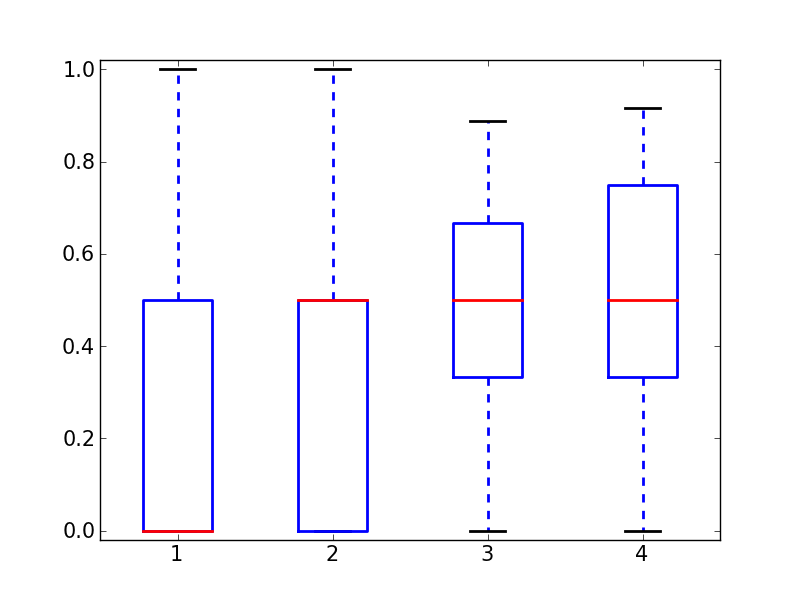
\includegraphics[width=0.45\textwidth, height=0.25\textwidth]{box_repimg.png}
%\miniskip
\label{fig:memo_t1}
}
\subfigure[]{
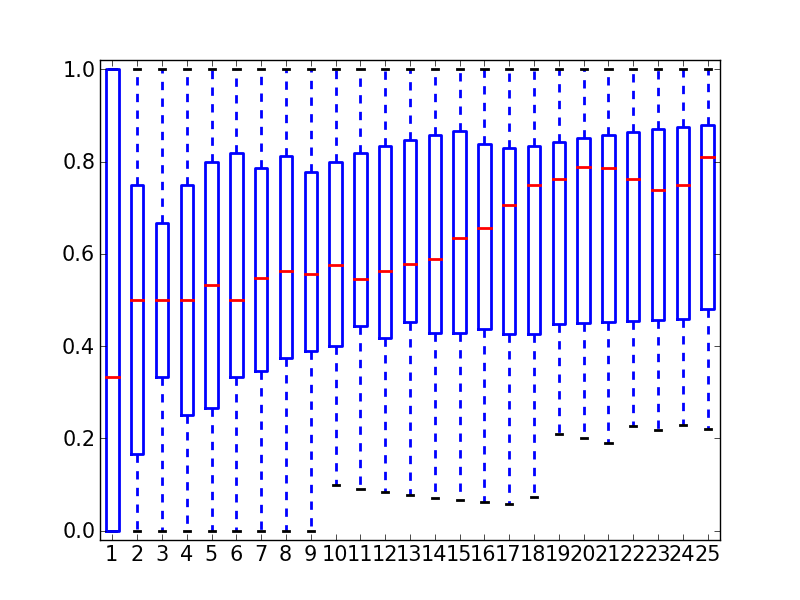
\includegraphics[width=0.45\textwidth, height=0.25\textwidth]{box_speciesimg.png}
%\miniskip
\label{fig:gene_t1}
}
\\
\subfigure[]{
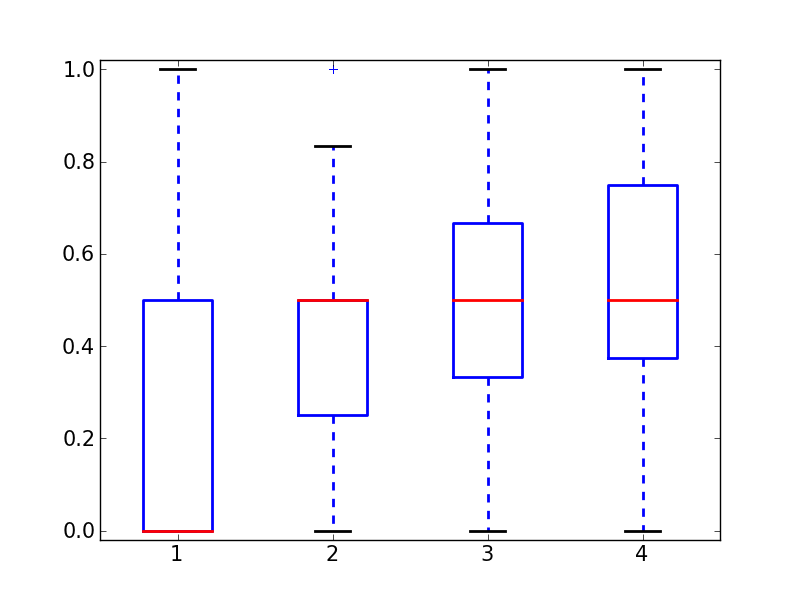
\includegraphics[width=0.45\textwidth, height=0.25\textwidth]{memo_t2.png}
%\miniskip
\label{fig:memo_t2}
}
\subfigure[]{
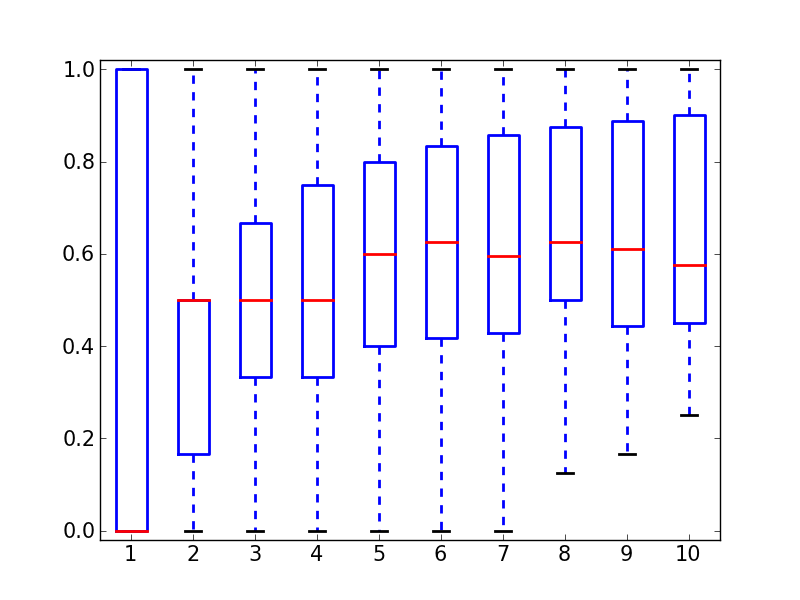
\includegraphics[width=0.45\textwidth, height=0.25\textwidth]{gene_t2.png}
%\miniskip
\label{fig:gene_t2}
}
\caption{The learning behavior of non-experts: memorizing (left) 
and generalization (right). Figures~\ref{fig:memo_t1} and~\ref{fig:gene_t1} are result of Experiment 1;
Figure~\ref{fig:memo_t2} and~\ref{fig:gene_t2} are result of Experiment 2.}
\label{fig:learn}
%\vspace*{-\baselineskip}
\end{figure*}
%
The numbers in Table~\ref{tab:effect} confirms that there is a significant difference 
between the scores achieved with the first label and those achieved over time, in both 
experiments non-experts can learn and improve their labels over time. 
They do not only learn to provide more accurate labels for images that they have seen 
before, but also for similar images, i.e., different images that contain species that they have seen before. 


\fi

%\todo{Maybe to the conclusion: While we can not conclusively say that the annotators learn from the 
%system feedbacks, as many other factors can contribute to their improvement, e.g., 
%they may get used to the quality of the images over time, we do believe that the system feedback is 
%a major reason that the annotators are able to improve their performance. Some annotators 
%explicitly explained how they approach to achieve higher points as well as their experience of 
%memorizing the options that give them highest points. In order to have a better understanding of 
%how annotators learn during the annotation process and what makes the learning most effective, 
%more controlled experiments are needed. This is however out of the scope of this paper.} 





%\begin{table}
%\centering
%\begin{tabular}{@{}l@{~~}l@{~}l@{~~~}l@{~}l@{~~~}l@{~}l@{~~~}l@{~}l@{}}
%\hline
%& \multicolumn{2}{c}{E1} & \multicolumn{2}{c}{E2} & \multicolumn{2}{c}{E3} & \multicolumn{2}{c}{E*} \\
%& Avg. $\kappa$ & Sdv. & Avg. $\kappa$ & Sdv. & Avg. $\kappa$ & Sdv. & Avg. $\kappa$ & Sdv. \\
%\hline
%E1 & - & - & - & - & - & - & 0.59 & 0.01 \\
%E2 & 0.55 & 0.008 &  - & - & - & - & 0.55 & 0.001\\
%E3 & 0.48 & 0.008 & 0.67 & 0.006 & - & -  & 0.52 & 0.07 \\
%U.random & 0.51 & 0.03 & 0.53 & 0.03 & 0.45 & 0.03 & - & - \\ 
%U.Vote  & 0.35 & 0.009 & 0.34 & 0.004 & 0.31 & 0.006 & 0.30 & 0.01\\
%U.MAP & 0.58 & 0.01 & 0.55 & 0.001 & 0.49 & 0.006 & 0.46 & 0.03  \\ 
%U.MVote & 0.62 & 0.01 & 0.65 & 0.006 & 0.55 & 0.009 \\
%U.Zscore & 0.55 & 0.009 & 0.57 & 0.005 & 0.49 & 0.008 \\
%\hline
%\end{tabular}
%\caption{Cohen's kappa for measuring annotation agreement at species level.}
%\label{tab:species_agree}
%\end{table}
%
%\begin{table}
%\centering
%\begin{tabular}{@{}l@{~~}l@{~}l@{~~~}l@{~}l@{~~~}l@{~}l@{~~~}l@{~}l@{}}
%\hline
%& \multicolumn{2}{c}{E1} & \multicolumn{2}{c}{E2} & \multicolumn{2}{c}{E3} & \multicolumn{2}{c}{E*} \\
%& Avg. $\kappa$ & Sdv. & Avg. $\kappa$ & Sdv. & Avg. $\kappa$ & Sdv. & Avg. $\kappa$ & Sdv. \\
%\hline
%E1 & - & - & - & - & - & - & 0.71 & 0.01 \\
%E2 & 0.85 & 0.004 &  - & - & - & - & 0.66 & 0.01\\
%E3 & 0.75 & 0 & 0.76 & 0.0001 & - & -  & 0.83 & 0.01 \\
%U.random & 0.73 & 0.03 & 0.71 & 0.03 & 0.62 & 0.03 & - & -\\
%U.Vote  & 0.53 & 0.01 & 0.49 & 0.12 & 0.47 & 0.009 & 0.41 & 0.01\\
%U.MAP & 0.83 & 0.004 & 0.78 & 0 & 0.70 & 0 & 0.69 & 0.01  \\ 
%U.MVote & 0.83 & 0.008 & 0.81 & 0.01 & 0.72 & 0.009\\
%U.Zscore& 0.82 & 0.005 & 0.78 & 0.003 & 0.69 & 0.0001\\
%\hline
%\end{tabular}
%\caption{Cohen's kappa for measuring annotation agreement at family level. }
%\label{tab:family_agree}
%\end{table}


%\begin{itemize}
%\item Agreement between 3 experts: Fliess' kappa for multi-rater agreement.
%\item At species level, sometimes experts assign multiple labels to a single image, including cases such as
%they are not sure between species A and B as well as cases where they assign labels at family level.
%To cope with this situation, we randomly choose one of the multiple labels a biologist assigned to an image. 
%We repeat this process for 1000 times and report the average as well as standard deviation of 
%Fleiss' kappa calculated in this way. The agreement calculated this way is conservative.
%\item We look at both species level and family level. 
%\item To measure agreement between expert and players, we aggregate player judgement to a single
%rating of the candidate categories. Then we replace one of the 3 experts using this aggregated
%player rating and calculate the agreement.
%\item We take the candidates with the highest rating scores as the labels assigned by the players. 
%\end{itemize}

%\begin{table}
%\centering
%\begin{tabular}{@{}l@{~~}l@{~~}l@{~~}l@{~~}l@{}}
%\hline
%Agreement & \multicolumn{2}{c}{Species} & \multicolumn{2}{c}{Family}\\
%& Avg. $\kappa$& Stdv. & Avg. $\kappa$ & Stdv.\\ 
%\hline
%Expt. vs. Expt & 0.56 & 0.005 & 0.78 & 0.001\\
%\hline
%U.MAP vs. Expt$^{1,2}$& 0.57 & 0.002 & 0.74 & 0\\
%U.MAP vs. Expt$^{1,3}$& 0.51 & 0.005 & 0.76 & 0.001\\
%U.MAP vs. Expt$^{2,3}$& 0.56 & 0.004 & 0.82 & 0.002\\
%\hline
%U.Vote vs. Expt$^{1,2}$& 0.43 & 0.003 & 0.56 & 0.006\\
%U.Vote vs. Expt$^{1,3}$& 0.37 & 0.004 & 0.58 & 0.006\\
%U.Vote vs. Expt$^{2,3}$& 0.41 & 0.004 & 0.61 & 0.008\\
%\hline
%\end{tabular}
%\caption{Fliess' kappa for agreement, 1000 runs}
%\end{table}
 % results and discussion 
\section{Conclusion}
\label{sec:con}
We converted an image labeling task that requires extensive domain knowledge into an 
image matching game that is based on visual similarity comparison only.        
%and automatic feedback only. (automatic feedback is feedback without ground truth.)
%To be able to study the performance of players independently from the method used to select the 
%candidate labels,  we only used images already labeled by experts. 
%We first studied the performance of the players under the condition that the correct labels 
%(according to the experts) were always presented among the candidate labels. 
%
%The result 
When the correct labels are always presented among the candidate labels, 
non-experts can play this game rather well: 
domain experts agree as often with the aggregated game labels as they agree with each other's labels. 
Users learn while playing to the extent that they perform better not only when they later see the same image again, 
but also when they later see different images from the same species.
%
When the game is played under the more realistic condition that the correct label is not always presented, 
performance of novice users drops, but players that had played the 
game before still performed as good as under the ideal condition. 
Also under this condition, players still learned in terms of memorization and generalization.
%We confirmed that by converting a recognition problem to a visual similarity comparison problem, 
%non-experts can perform certain recognition tasks in specialists' domain without any domain knowledge.

%Now let us go back to the question we set out to address -- Do you need an expert in the crowd? 
%Based on what we have learnt in this study, the answer is mixed. 
%We see that the non-experts \emph{can} replace the experts to some extent if they have been trained
%with experts' feedback for sufficient time. 


A number of directions are left to be explored in the future. 
%
We used feedback from the experts, while in 
practice, the game will rely on automatic feedback or peer-agreement.
The influence of feedback quality on users' performance and learning behavior
is yet to be studied. 
%
%Further, in this study we addressed the question ``Can users learn?",  without further investigating how they learn
%and what makes them learn. 
%
Similarly, components within our labeling system such as the selection of candidates 
in practice will have to rely on automatic methods. While our user study have provided insights
into how these components influence user performance, it remains unexplored how these should be integrated
as a full fledged interactive system. 
%
Finally, we need to investigate how our approach can be extended to other domains such as medical image annotation. 


%Unfortunately, disagreement among players on a specific image leads to more unreliable data, even in the best performing aggregation method that we used. Having more players judge such images does not change this (? is this true ?). Picking an good aggregation method is important: in our case, the normalized voting method made the aggregated results worse than picking a single random judgement for each image.

%We also found that disagreement among experts is not correlated to disagreement among players. 
%In cases where experts disagree, but players show high agreement, this does not necessarily mean 
%that players agree on the correct answer. Again, in a real world setting with unlabeled images, 
%these cases are hard to detect automatically.

%The limitation of the study.

%\todo{What do we learn? 1) aggregation methods matter. 2) K - it's an ideal case, it matters. 3) entropy of the labels can imply the difficulty of the images.
%4) things difficult for experts also difficult for users?}

 % conclusion 

\ifanon
\else
%\miniskip
\section*{Acknowledgements}
This research was funded by European Commission FP7 grant 257024, in the Fish4Knowledge project (www.fish4knowledge.eu).
\fi

\renewcommand{\bibsection}{\section{\mbox{References}}}
\setlength{\bibsep}{1pt}
\bibliographystyle{abbrvnat}
%\footnotesize
\bibliography{oair2013-crowdsourcing}

\end{document}

